\documentclass[11pt,twoside]{article}
\addtolength{\textwidth}{0.5in}
\usepackage{epsfig,amsfonts,color}
\usepackage{amsmath}
\bibliographystyle{plain}
\usepackage{amssymb, palatino, geometry,url}
\usepackage{algorithmic}
\usepackage[noresetcount,lined,boxed]{algorithm2e} % ... for algorithms
\usepackage[colorlinks=true,linkcolor=blue,citecolor=blue,urlcolor=blue]{hyperref}
\geometry{letterpaper,
          left       = 0.9in,
          right      = 0.9in,
          top        = 0.9in,
          bottom     = 0.9in}
\linespread{1.2}

\usepackage{fancyhdr}
\usepackage{enumerate}
\usepackage{float}
\usepackage{subcaption}
\usepackage{graphicx}
\usepackage{caption}
\newcommand{\twopart}[4]
{
	\left\{
		\begin{array}{ll}
			#1 & \mbox{ } {\textrm{#2}} \\
			#3 & \mbox{ } {\textrm{#4}}
		\end{array}
	\right.
}

\newcommand{\N}{\mathbb{N}}
\newcommand{\Z}{\mathbb{Z}}
\newcommand{\Q}{\mathbb{Q}}
\newcommand{\R}{\mathbb{R}}
\title{Optimization Model for Operating Battery Systems in Multi-Level Electricity Markets}
\date{Ranjeet Kumar}
\author{CBE 750 Course Project}
\begin{document}
\maketitle

\section{Problem Statement}
The rechargeable Li-ion batteries can be inter-connected to the power grid to provide electricity and regulation services to the grid. By electricity services we mean that the batteries can provide power to or draw power from the grid and by regulation services we mean that the power drawn from or provided by the grid to the batteries can be regulated within a certain regulation up and regulation down capacity or a "regulation band" which the battery-owners bid for. The operator of the power grid (which is called an Independent System Operator or ISO) pays the battery-owners for both the electricity and regulation services. The goal for the battery-owners is to maximize the revenues generated from both the services.

The electricity markets in California are organized in three levels of time - (1) Day-ahead market, (2) Quarter-hourly market, (3) Real-time market. The  day-ahead market has the time scale of 1 hour, quarter-hourly market has the time scale of 15 minutes and the real-time market has the time scale of 5 minutes. Here, for example, the time scale of the day-ahead market means that the electricity in day-ahead market is traded in intervals of 1 hour with the prices being constant in each interval of 1 hour and varying after the intervals. The price data in the three levels of energy markets for a day have been shown in Figure \ref{eprices}.
\begin{figure}[h!tp]
\centering
\begin{subfigure}[b]{0.32\textwidth} 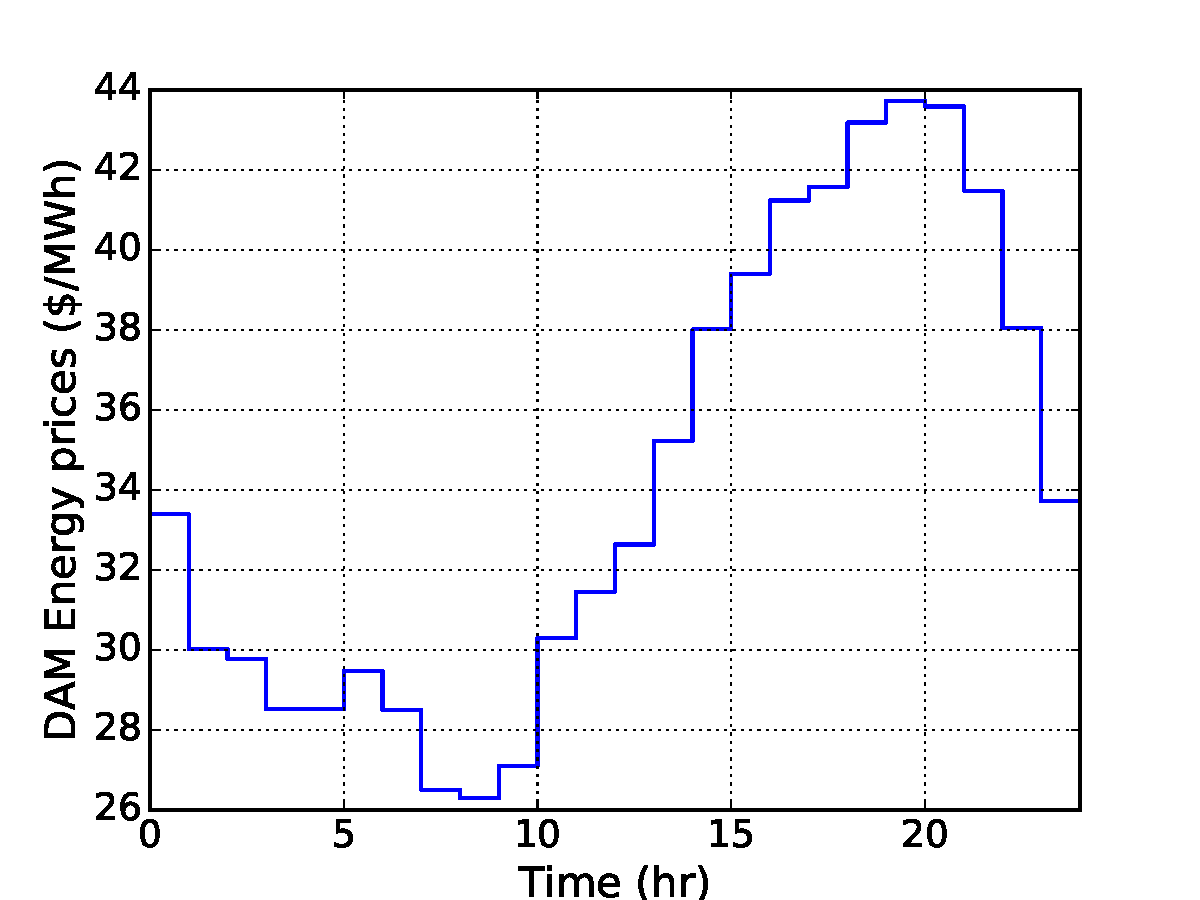
\includegraphics[width=\textwidth]{Figures/damprices.pdf} \caption{Day-ahead market}\label{damprices} \end{subfigure} \hfill
\begin{subfigure}[b]{0.32\textwidth} 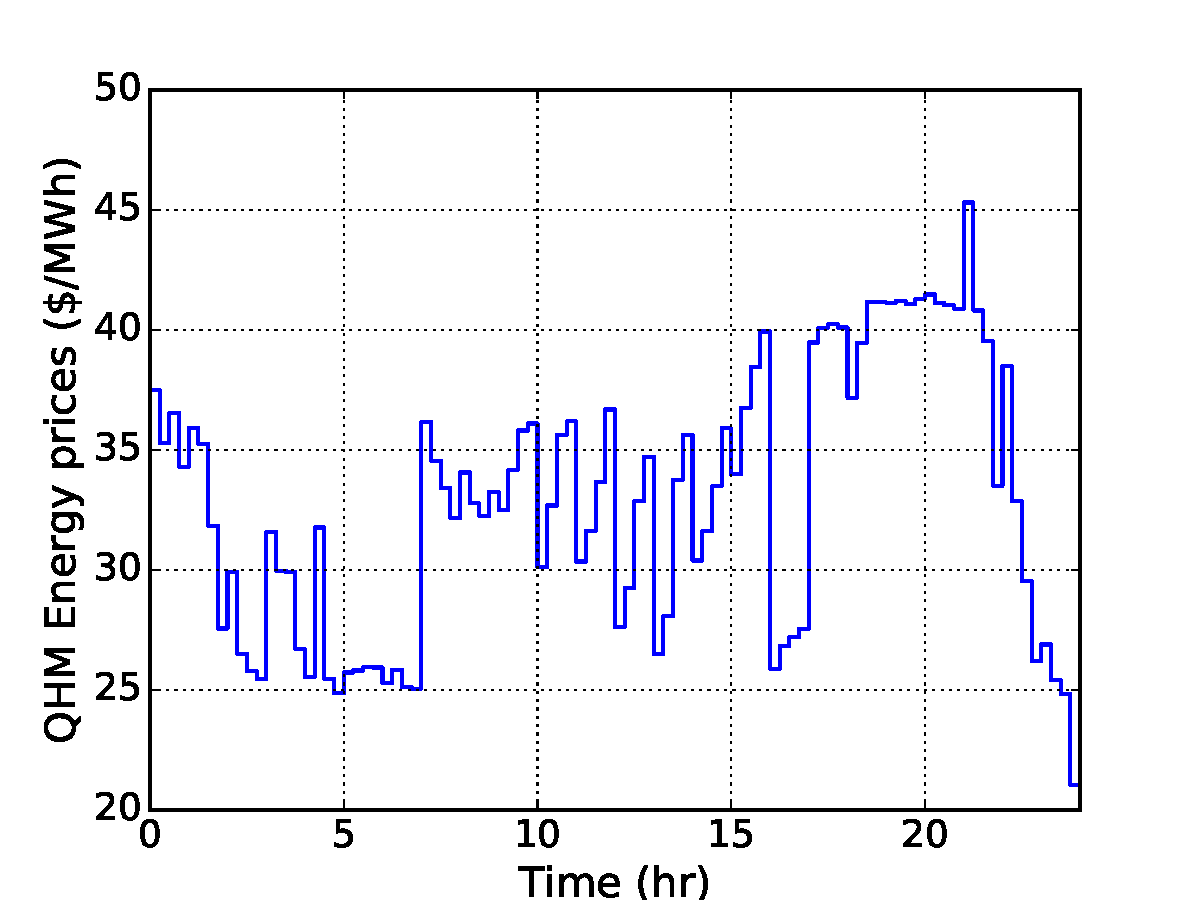
\includegraphics[width=\textwidth]{Figures/qhmprices.pdf} \caption{Quarter-hourly market}\label{qhmprices} \end{subfigure} \hfill
\begin{subfigure}[b]{0.32\textwidth} 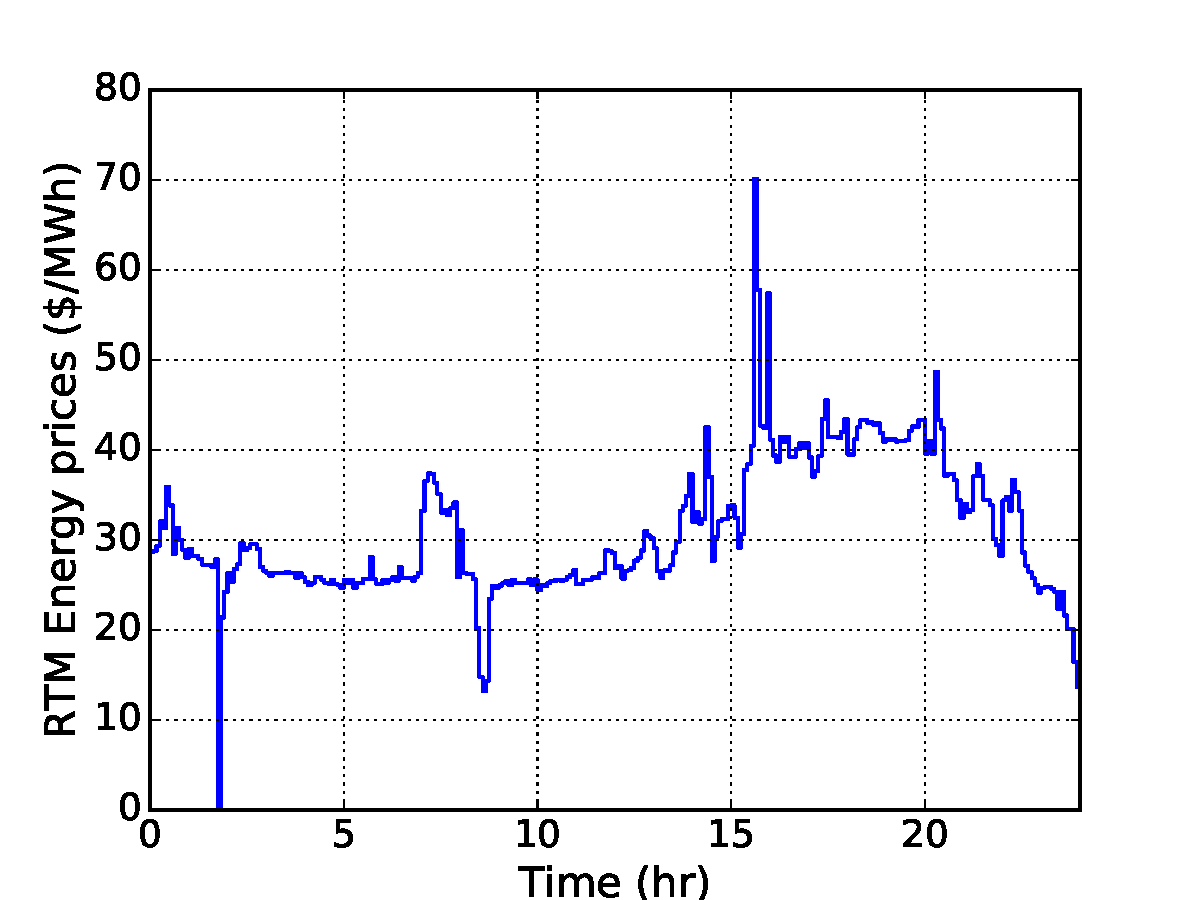
\includegraphics[width=\textwidth]{Figures/rtmprices.pdf} \caption{Real-time market}\label{rtmprices}\end{subfigure} \hfill
\caption{Energy prices in the markets in California}\label{eprices}
\end{figure}
We can observe that there are different frequencies of variation in energy prices in each of the three markets.

On the other hand, the regulation services are traded at two levels of time - (1) Day-ahead market and (2) Quarter-hourly market. The price data in the two levels of regulation markets for a day have been shown in Figure \ref{regprices}.
\begin{figure}[h!tp]
\centering
\begin{subfigure}[b]{0.49\textwidth} 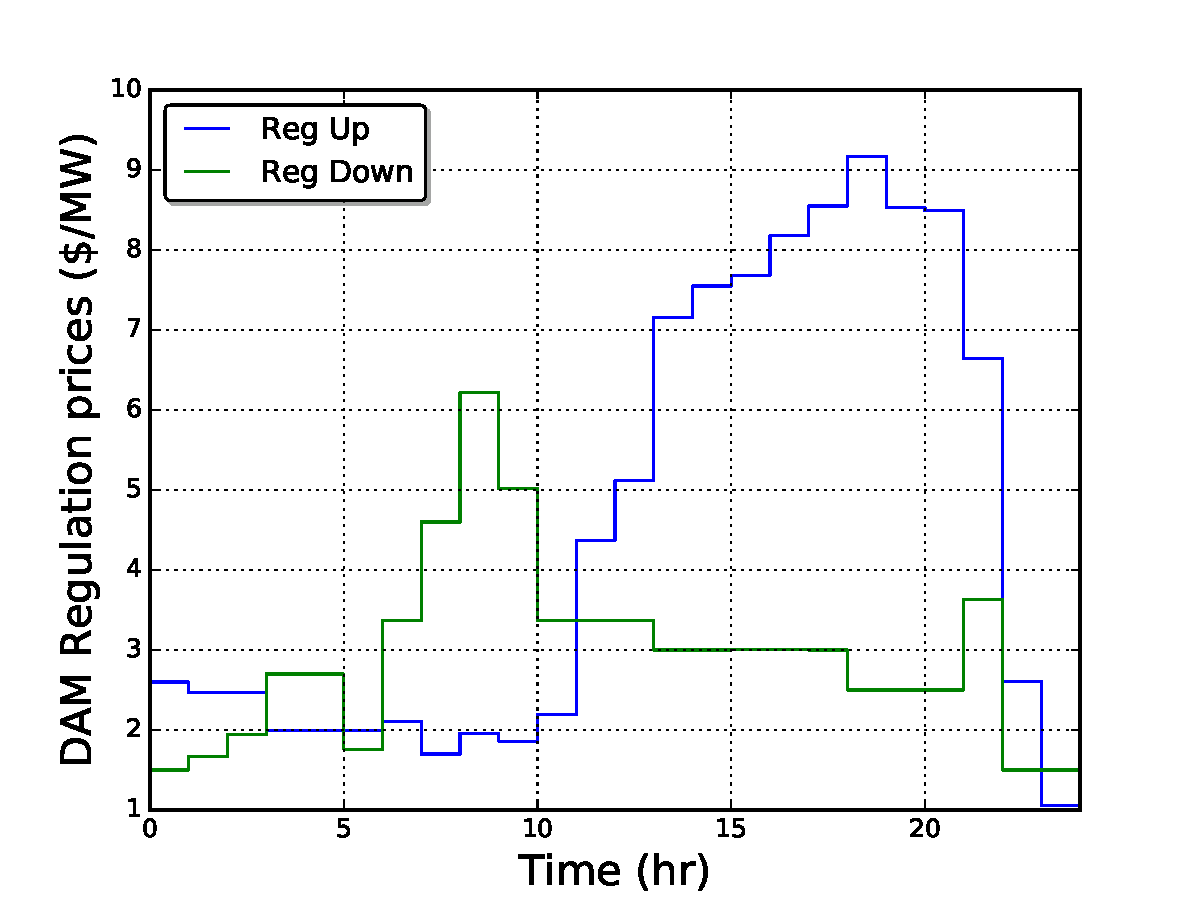
\includegraphics[width=\textwidth]{Figures/DAM_Reg_Price.pdf}\caption{Day-ahead market}\label{damregprices} \end{subfigure} \hfill
\begin{subfigure}[b]{0.49\textwidth} 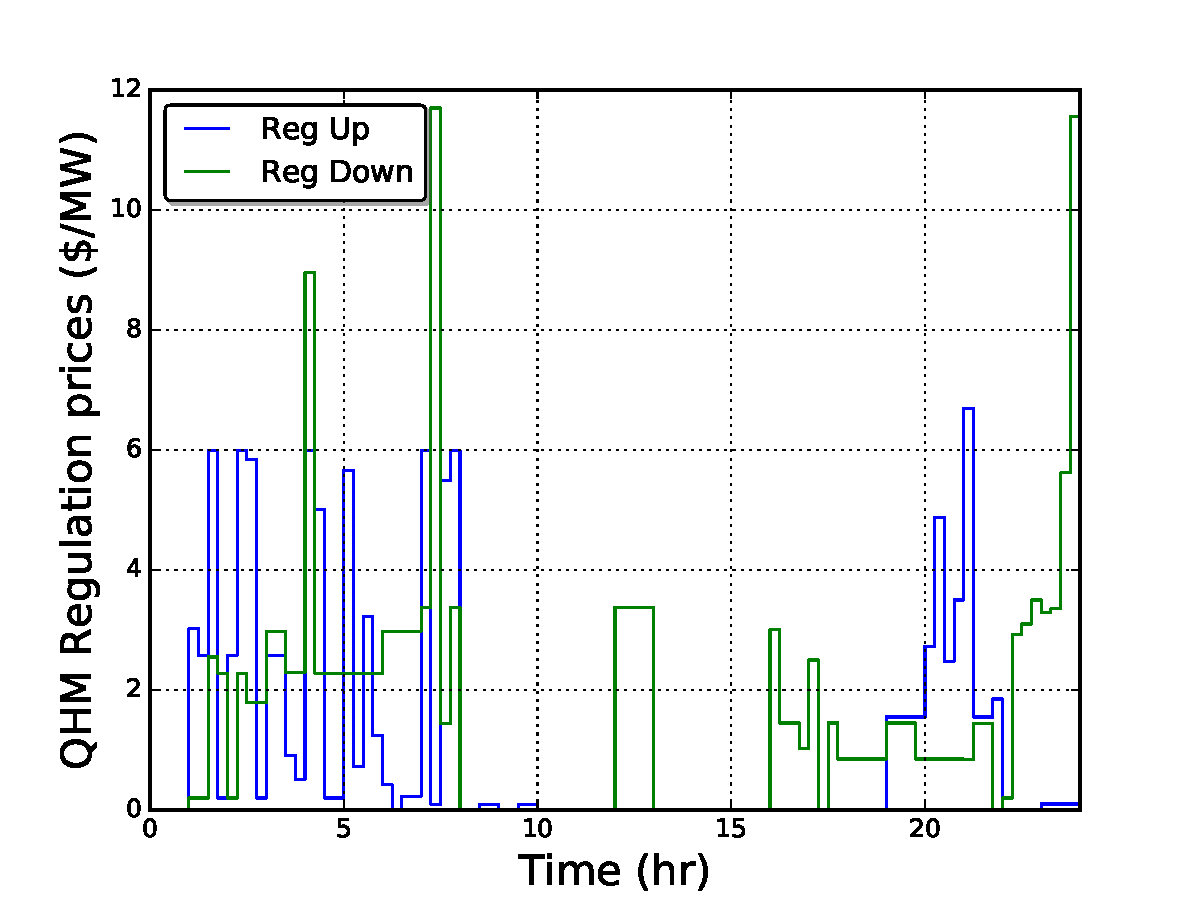
\includegraphics[width=\textwidth]{Figures/QHM_Reg_Price.pdf}\caption{Quarter-hourly market}\label{qhmregprices} \end{subfigure}
\caption{Regualtion prices in the regulation markets in California}\label{regprices}
\end{figure}

Cosidering the price data for a full year to be known (deterministic) we can solve the optimization problem to maximize the annual revenues by operating a battery in the power grid for the whole year. In this work, we aim to solve this deterministic optimization problem with two approaches:
\begin{enumerate}
\item Simultaneous approach: In this approach, we formulate a single giant optimization problem for a full year and solve it to produce the optimal power and regulation capacities that the battery should operate with in each time interval in all the three markets. 
\item Rolling (1 day) horizon approach: In this approach, we formulate an optimization problem for a day and solve it to produce the optimal power and regulation capacities for that day, then take the solutions at the end time-point of that day as the initial point for the next day, then formulate the optimization problem for the next day with those initial values and solve for the second day and sequentially we solve for the 365 days. It is called rolling horizon because in this approach we consider a horizon of 1 day and keep shifting the horizon to to the next day after solving the current day.
\end{enumerate}

At the end, we will compare the two solutions and investigate the advantages and disadvantages of the two approaches.

\section{Optimization problem formulation}
The abstract model is shown in the Figure \ref{model}. Note that the power of the battery can be negative when it is charging, that is when the battery is drawing power from the power grid.
\begin{figure}[h!tp]
\centering
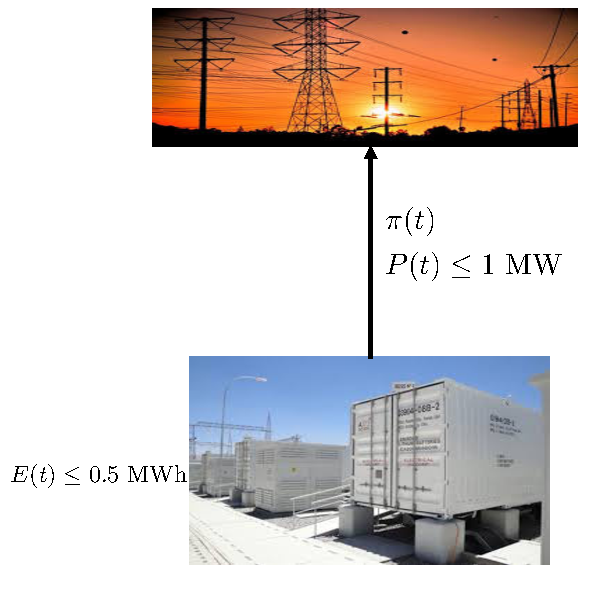
\includegraphics[width=3in]{Figures/model.pdf}
\caption{Battery connected to power grid}\label{model}
\end{figure}
The optimization model for each day can be formulated as follows:\\
\paragraph{Sets:}
\begin{subequations}
\begin{align}
R := \{1,..,n_r\},\; Q :=  \{1,..,n_q\},\; D :=  \{1,..,n_d\}
\end{align}
\end{subequations}
Here, R is the set of time indices for the real-time subintervals within each quarter-hour interval, so $n_r=3$, Q is the set of time indices for the quarter-hourly intervals within each hour interval, so $n_q=4$ and R is the set of time indices for the hourly intervals within each day, so $n_d=24$.\\
\paragraph{Indices:}
\begin{subequations}
\begin{align}
i \in R, \; j \in Q, \; k \in D
\end{align}
\end{subequations}
\paragraph{Constraints for each day in the model:}
\begin{subequations}
\begin{align}
&E_{1,1,1} = E_{0} + \eta (P_{i,j,k} + P_{j,k} + P_{k})\Delta t_r\\
&E_{n_r,n_q,n_d} \geq E_{end}
\end{align}
\label{eq1}
\end{subequations}
\vspace{-0.45in}
\begin{subequations}
\begin{align}
E_{i,j,k} =&\; E_{i-1,j,k}- \eta (P_{i,j,k} + P_{j,k} + P_{k})\Delta t_r\\
E_{1,j,k} =&\; E_{n_r,j-1,k}- \eta (P_{1,j,k} + P_{j,k} + P_{k})\Delta t_r\\
E_{1,1,k} =&\; E_{n_r,n_q,k-1}- \eta (P_{i,j,k} + P_{j,k} + P_{k})\Delta t_r
\end{align}
\label{eq2}
\end{subequations}
\vspace{-0.45in}
\begin{subequations}
\begin{align}
P_{i,j,k} + P_{j,k} + P_{k} + R^U_{j,k} + R^U_{k} \leq &\; P_{max}\\
P_{j,k} + P_{k} + R^U_{j,k} + R^U_{k} \leq &\; P_{max}\\
P_{k} + R^U_{k} \leq &\; P_{max}\\
P_{i,j,k} + P_{j,k} + P_{k} - R^D_{j,k} - R^D_{k} \geq &\; P_{min}\\
P_{j,k} + P_{k} - R^D_{j,k} - R^D_{k} \geq &\; P_{min}\\
P_{k} + R^D_{k} \geq &\; P_{min}
\end{align}
\label{eq3}
\end{subequations}\vspace{-0.45in}
\begin{subequations}
\begin{align}
0 & \leq E_{i,j,k} \leq E_{max}\\
-P_{max} & \leq P_{i,j,k} \leq P_{max}\\
-P_{max} & \leq P_{j,k}\phantom{i,} \leq P_{max}\\
-P_{max} & \leq P_{k}\phantom{i,j} \leq P_{max}\\
0 & \leq R^U_{j,k}\phantom{i,} \leq R_{max}\\
0 & \leq R^U_{k}\phantom{i,j} \leq R_{max}\\
0 & \leq R^D_{j,k}\phantom{i,} \leq R_{max}\\
0 & \leq R^D_{k}\phantom{i,j} \leq R_{max}
\end{align}
\label{eq4}
\end{subequations}\vspace{-0.45in}
\begin{subequations}
\begin{align}
Rev_E =& \sum_{i \in R} \sum_{j \in Q} \sum_{k \in D} \Delta t_r(\pi^E_{i,j,k}P_{i,j,k}) + \sum_{j \in Q} \sum_{k \in D}\Delta t_q(\pi^E_{j,k}P_{j,k}) + \sum_{k \in D}\Delta t_d(\pi^E_{k}P_{k})\\
Rev_R =& \sum_{j \in Q} \sum_{k \in D}\Delta t_m(\pi^U_{j,k}R^U_{j,k})+\sum_{k \in D}\Delta t_s(\pi^U_{k}R^U_{k}) + \sum_{j \in Q} \sum_{k \in D}\Delta t_m(\pi^D_{j,k}R^D_{j,k})+\sum_{k \in D}\Delta t_s(\pi^D_{k}R^D_{k})
\end{align}
\label{eq5}
\end{subequations}
Here, the decision variables are $E$, the energy of the battery at every time interval, $P$, the net power of the battery going to the power grid in the three markets, $R^U$, the regulation up capacities in the two levels of regulation markets, $R^D$, the regulation down capacities in the two levels of regulation markets and $Rev^E$ and $Rev^R$, the revenues from the energy and regulation markets respectively. The three subscripted indices in $P$, $R^U$ and $R^D$ variables mean that they are for the real-time market, the two subscripted indices in $P$, $R^U$ and $R^D$ variables mean that they are for the quarter-hourly market and the one subscripted index in $P$, $R^U$ and $R^D$ variables mean that they are for the day-ahead market. $\pi$'s are the prices which are known parameters in the model, the superscript on $\pi$ denotes the quantity which it is the price of and subscripts on $\pi$ denotes the level of market of which it is the price.

\begin{figure}[h!tp]
\centering
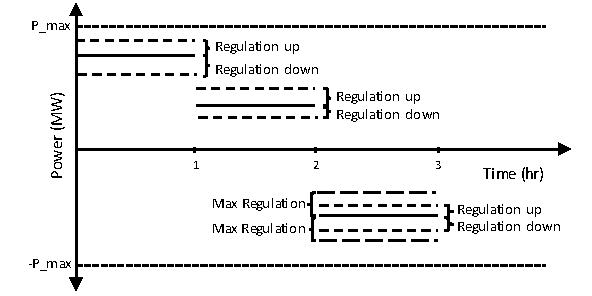
\includegraphics[width=4.5in]{Figures/regexample.pdf}
\caption{An example showing the regulation up and down capacitites in day-ahead market}\label{regexample}
\end{figure}
 
The constraints in Eq. \ref{eq1} are to define the energy of the battery at the first time interval and at the end time of the day. The constraints in Eq. \ref{eq2} are the energy balance equations at each time intervals. The constraints in Eq. \ref{eq3} are to ensure that the power of the battery after adding (or subtracting) the regulation up (or down) capacities does not go beyond the maximum allowable power of the battery at each time intervals, as shown in the Figure \ref{regexample}. The constraints in Eq. \ref{eq4} provide the upper and lower bounds of each variables at each interval. The constraints in Eq. \ref{eq5} calculate the revenues from the energy markets and the regulation markets.

In the rolling horizon approach, this problem can be solved sequentially with the added constraint for the intermediate days that the end point solutions for the current day will be the values of those variables at the first time point of the next day. Solving in this fashion will finally result in the optimal values of power and regulation capacities in each level of market for each day.

In the simultaneous approach, we formulate the optimization problem for the full year by introducing another index (subscript) for the day in all the variables and prices. That problem can then be solved to produce the optimal values of power and regulation capacities for each time interval for the whole year at once.


\section{Results}
\subsection{Simutaneous approach}
The problem was formulated in Julia programming language with JuMP modeling language and was solved with Gurobi solver. The problem is a linear program whose size is as follows:
\begin{itemize}
\item 1,103,761 variables
\item 911,041 linear constraints
\end{itemize}
The computation time to solve the problem was slightly over 20 seconds.

The optimal revenues obtained with this approach were as follows:
\begin{itemize}
\item Total annual revenues: \$293,125
\item Revenues from energy sale: \$201,281
\item Revenues from regulation: \$91,844.
\end{itemize}

The optimal battery power to the power grid, the optimum regulation up and down capacities, the optimum battery performance curves and the revenue profiles during one of the days (day 91) in the year have been shown in Figures \ref{psim}, \ref{regsim}, \ref{perfsim} and \ref{revsim} respectively.
\begin{figure}[h!tp]
\centering
\begin{subfigure}[b]{0.49\textwidth} 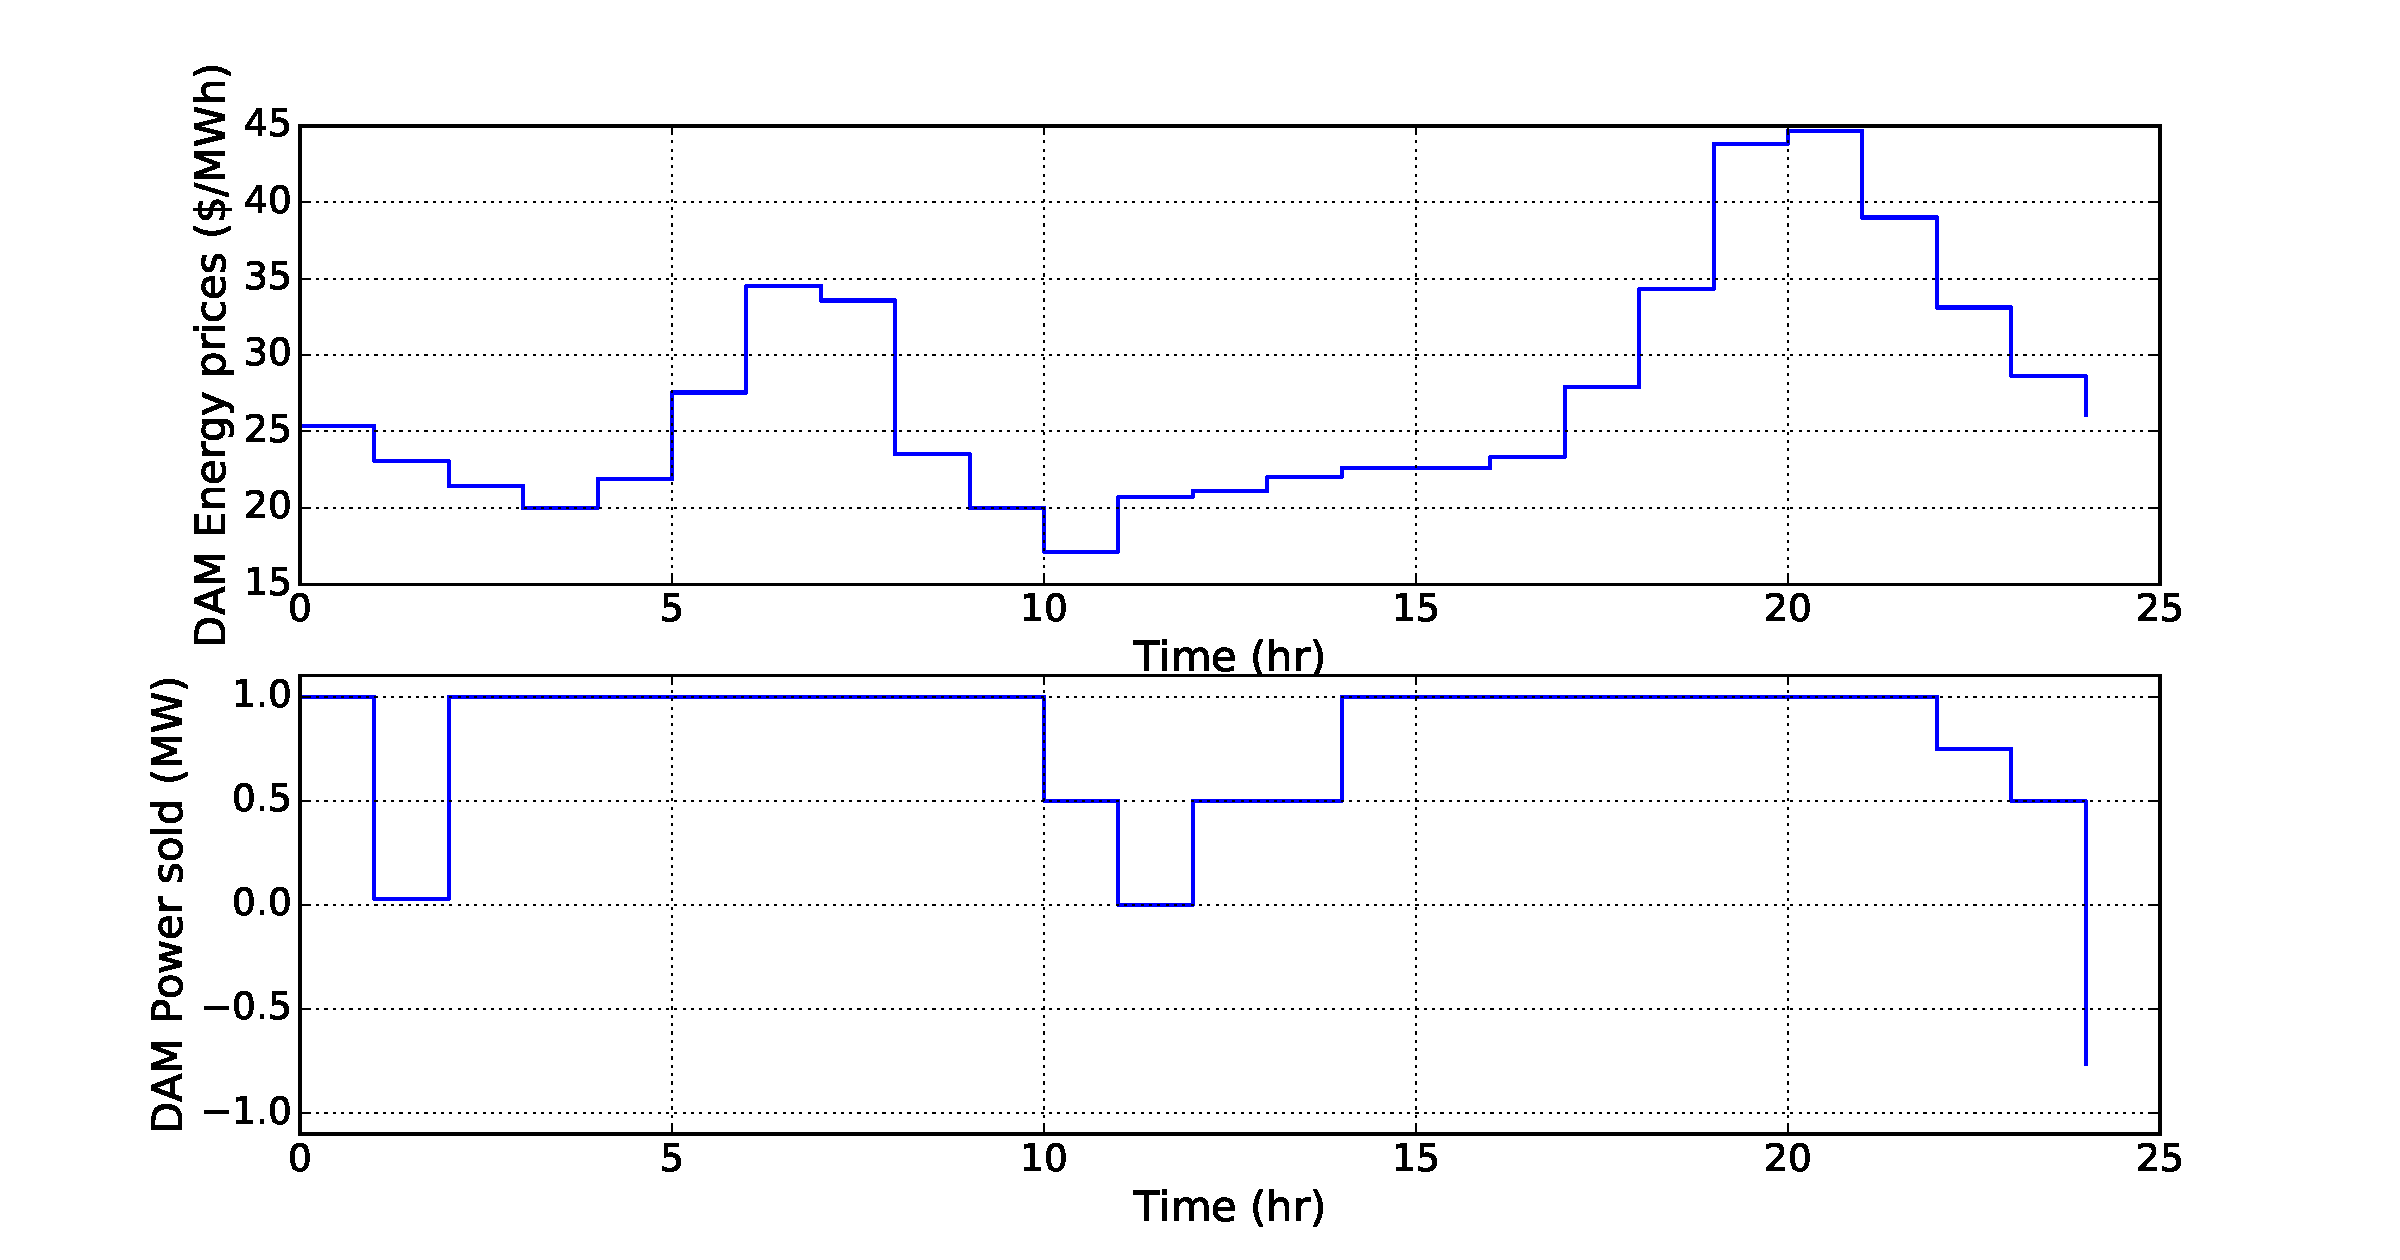
\includegraphics[width=\textwidth]{Figures/Plots/Simultaneous/DAM_P.pdf} \caption{Day-ahead market}\label{dampsim} \end{subfigure} \hfill
\begin{subfigure}[b]{0.49\textwidth} 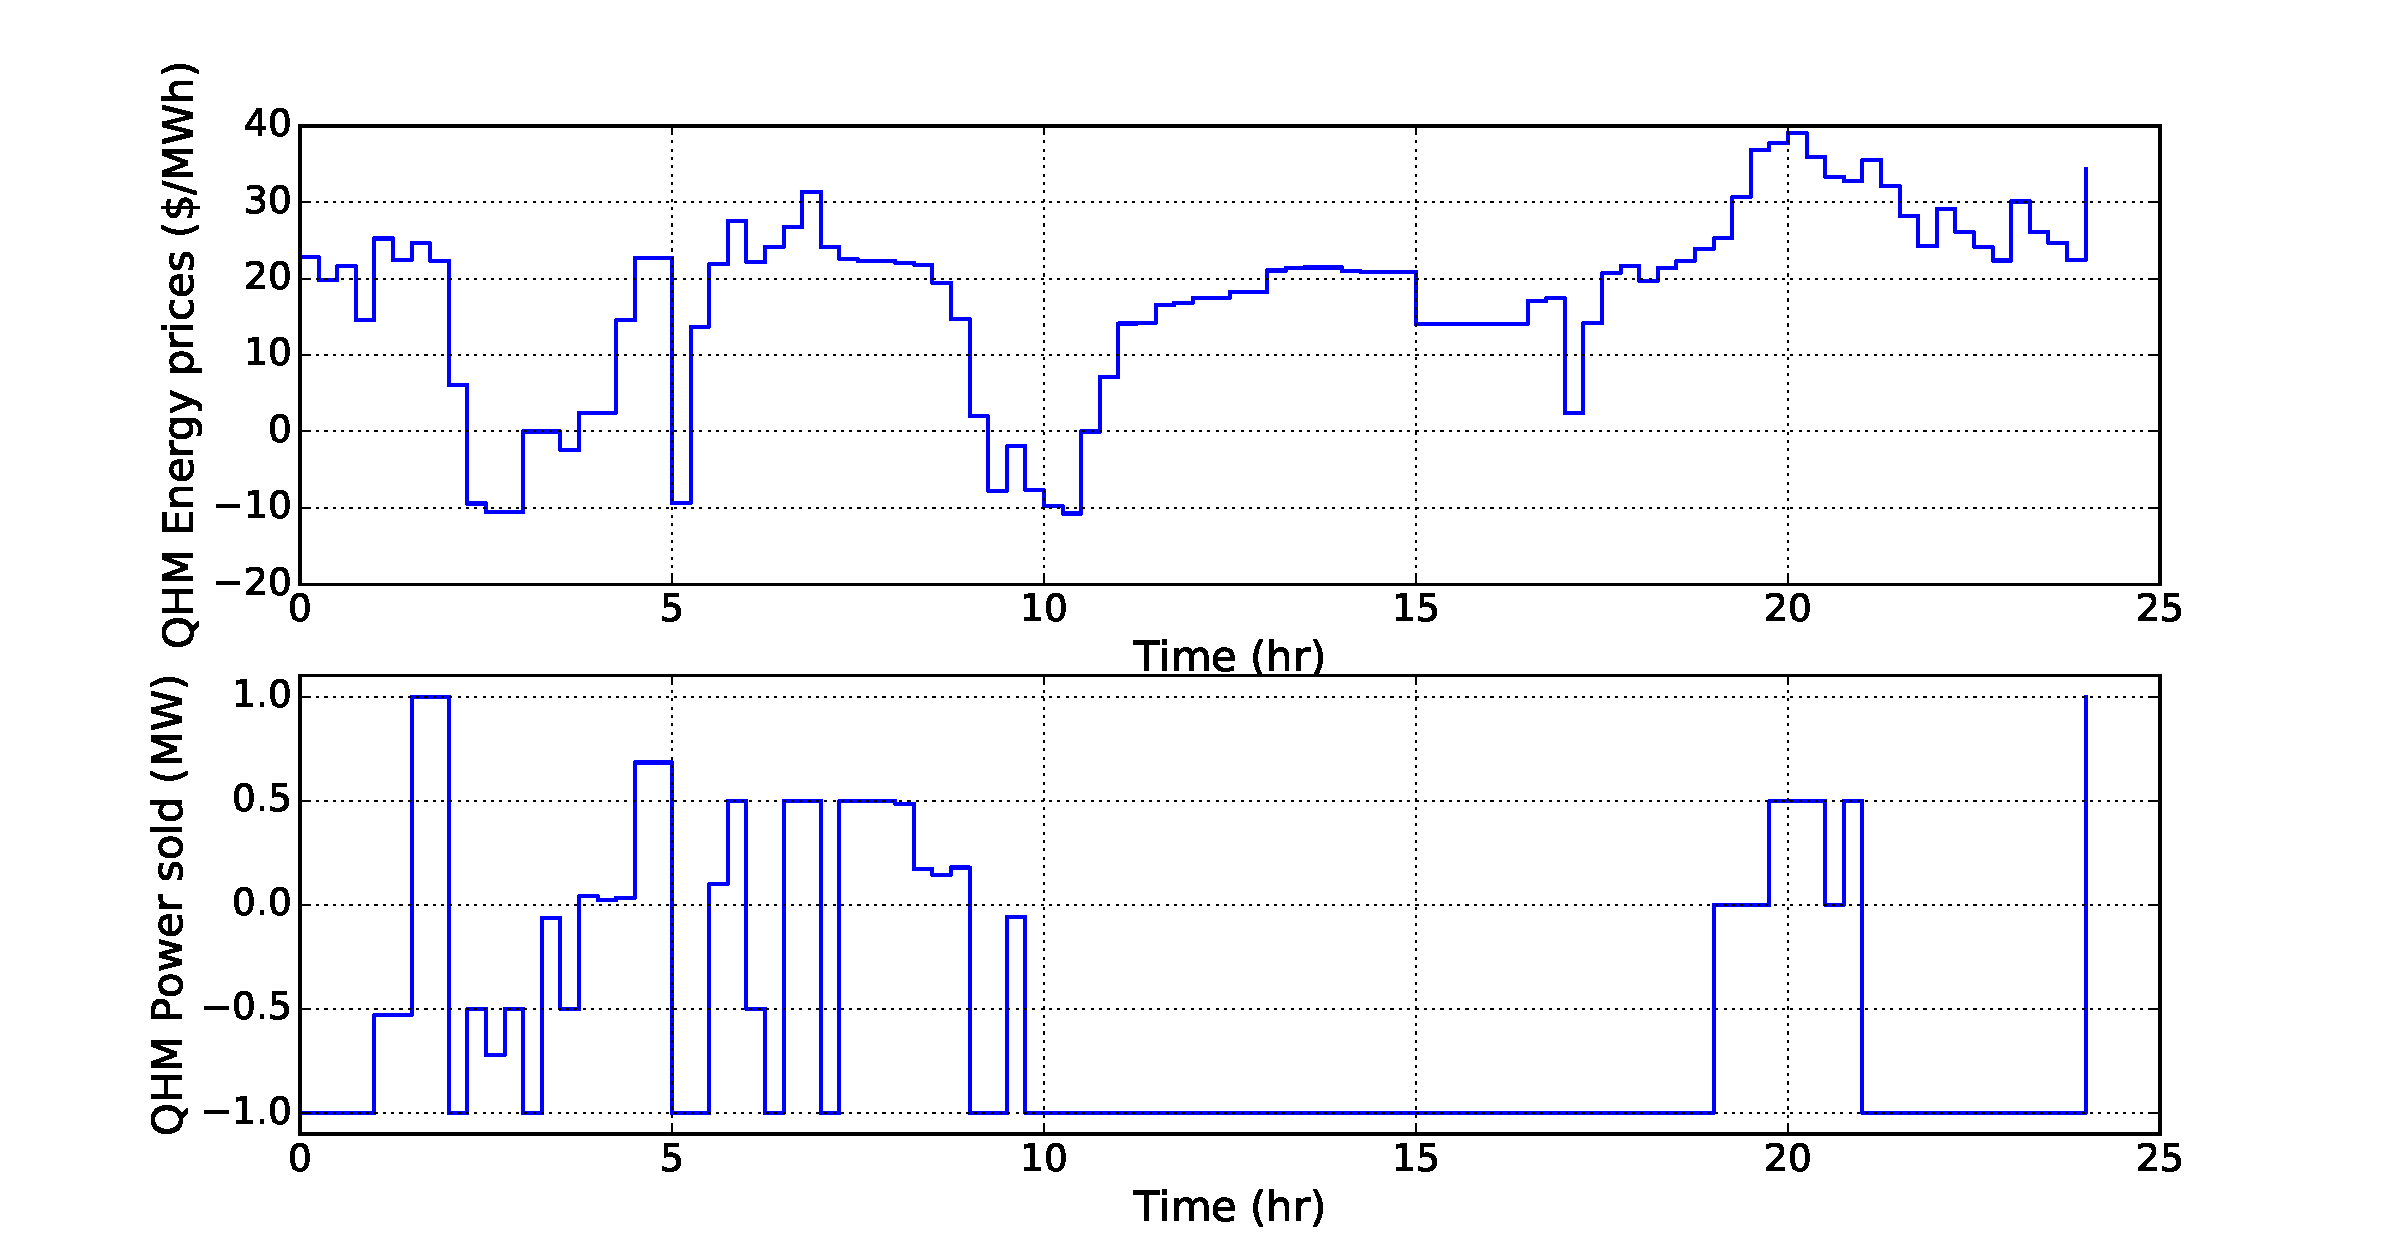
\includegraphics[width=\textwidth]{Figures/Plots/Simultaneous/QHM_P.pdf} \caption{Quarter-hourly market}\label{qhmpsim} \end{subfigure} \hfill
\begin{subfigure}[b]{0.49\textwidth} 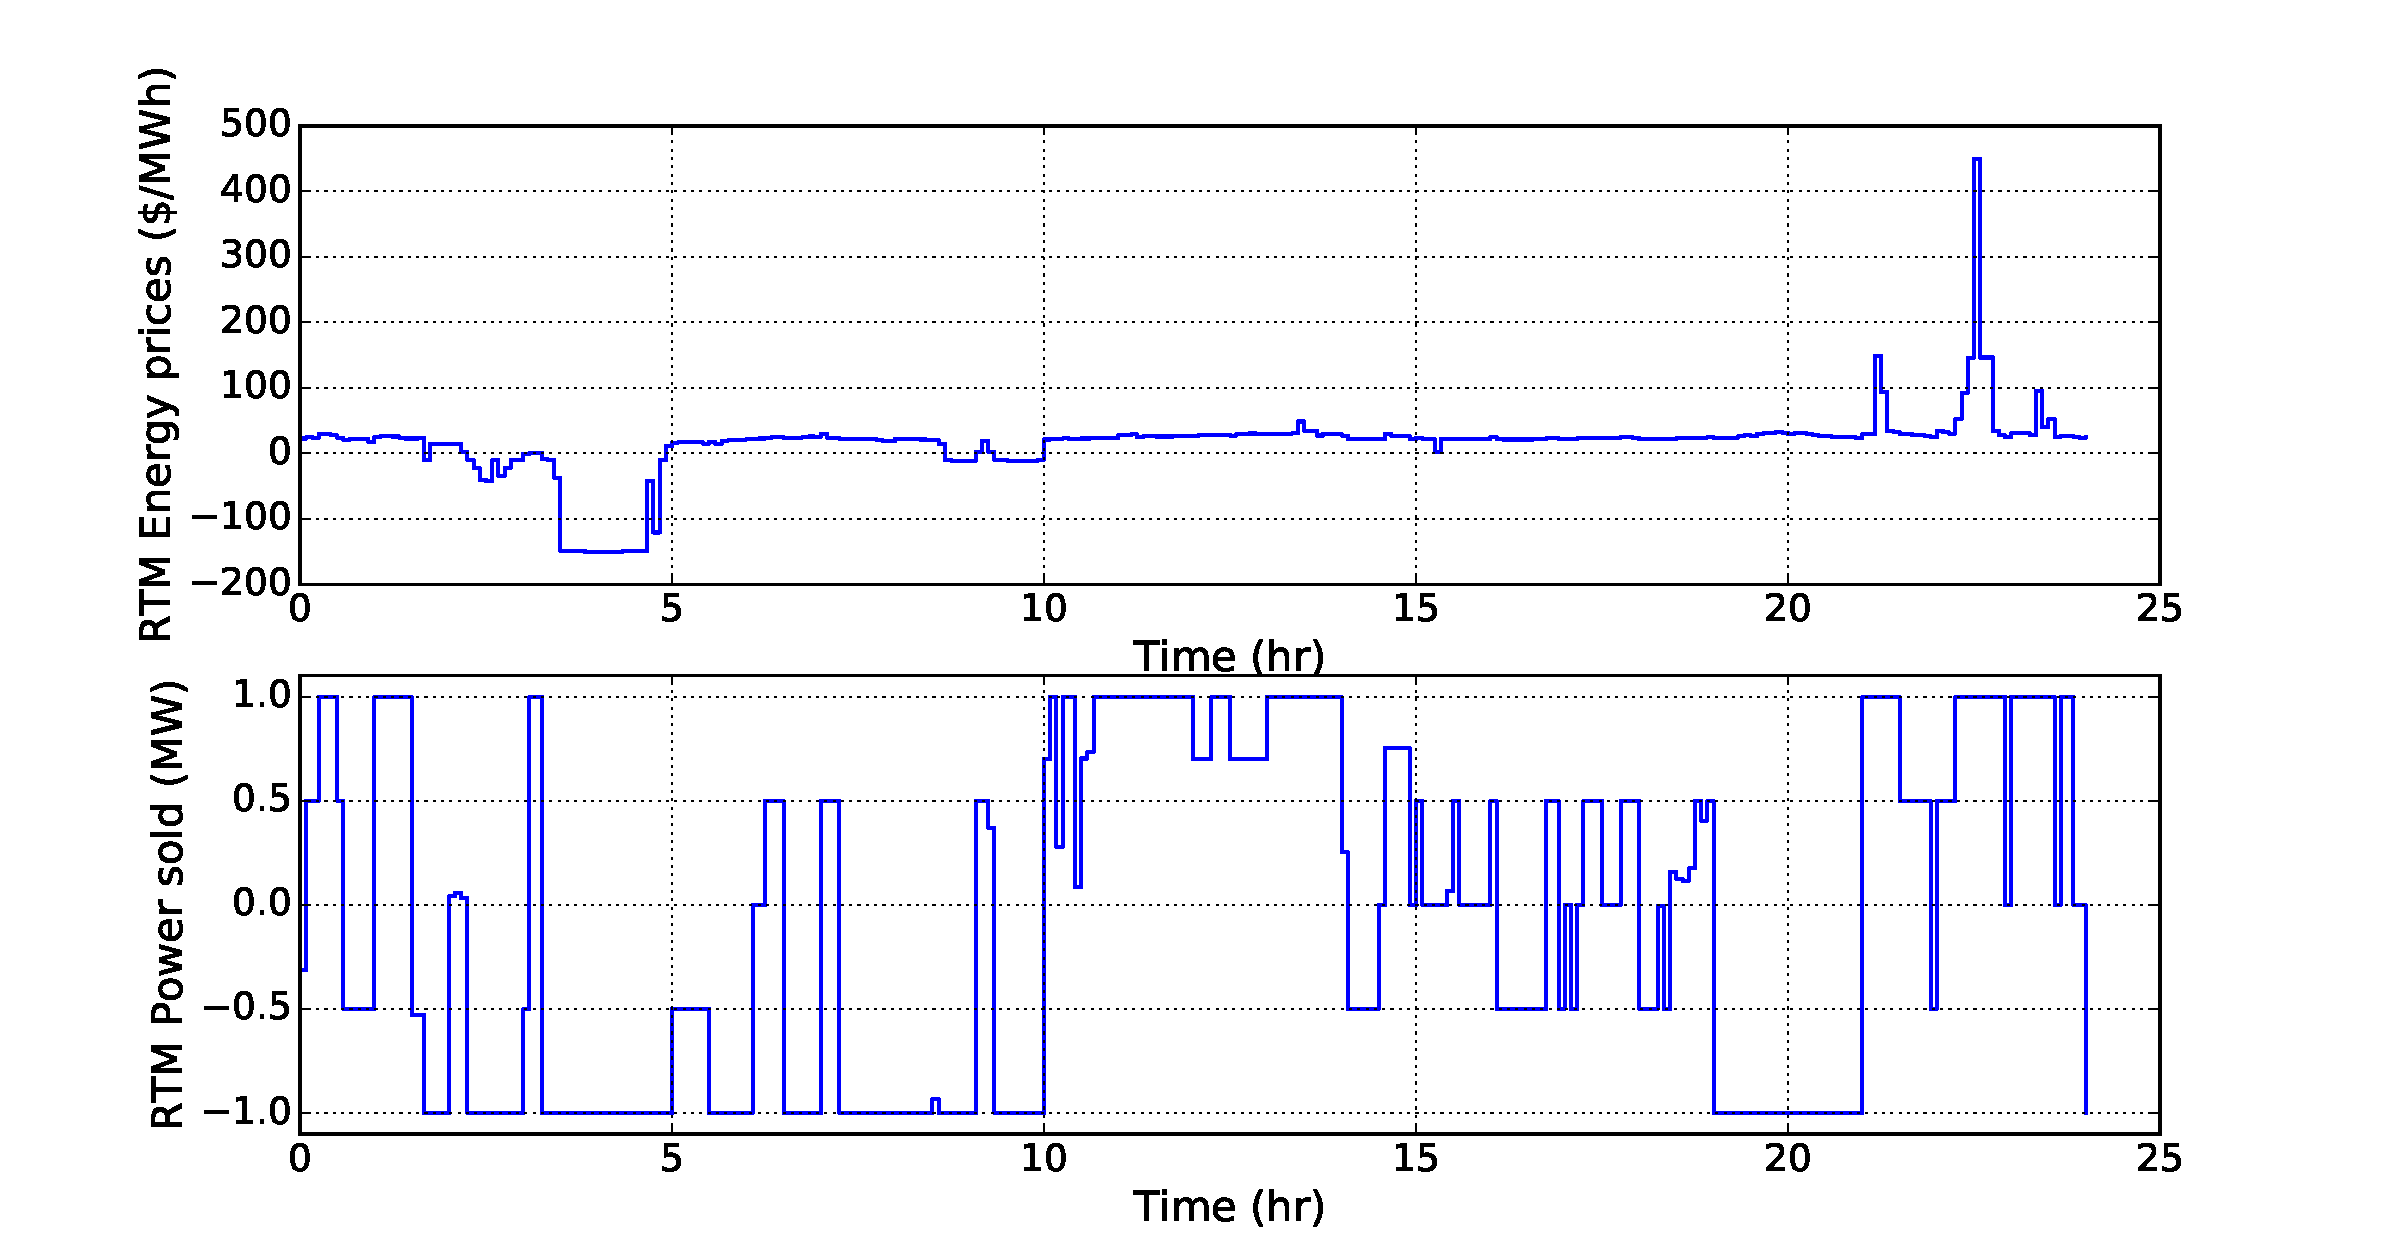
\includegraphics[width=\textwidth]{Figures/Plots/Simultaneous/RTM_P.pdf} \caption{Real-time market}\label{rtmpsim}\end{subfigure} \hfill
\caption{Optimal power obtained using simultaneous approach (shown only for day 91)}\label{psim}
\end{figure}
\begin{figure}[h!tp]
\centering
\begin{subfigure}[b]{0.49\textwidth} \includegraphics[width=\textwidth]{Figures/Plots/Simultaneous/DAM_Reg.pdf} \caption{Day-ahead market}\label{damregsim} \end{subfigure} \hfill
\begin{subfigure}[b]{0.49\textwidth} \includegraphics[width=\textwidth]{Figures/Plots/Simultaneous/QHM_Reg.pdf} \caption{Quarter-hourly market}\label{qhmregsim} \end{subfigure} \hfill
\caption{Optimal regulation capacities obtained using simultaneous approach (shown only for day 91)}\label{regsim}
\end{figure}
\begin{figure}[h!tp]
\centering
\begin{subfigure}[b]{0.49\textwidth} 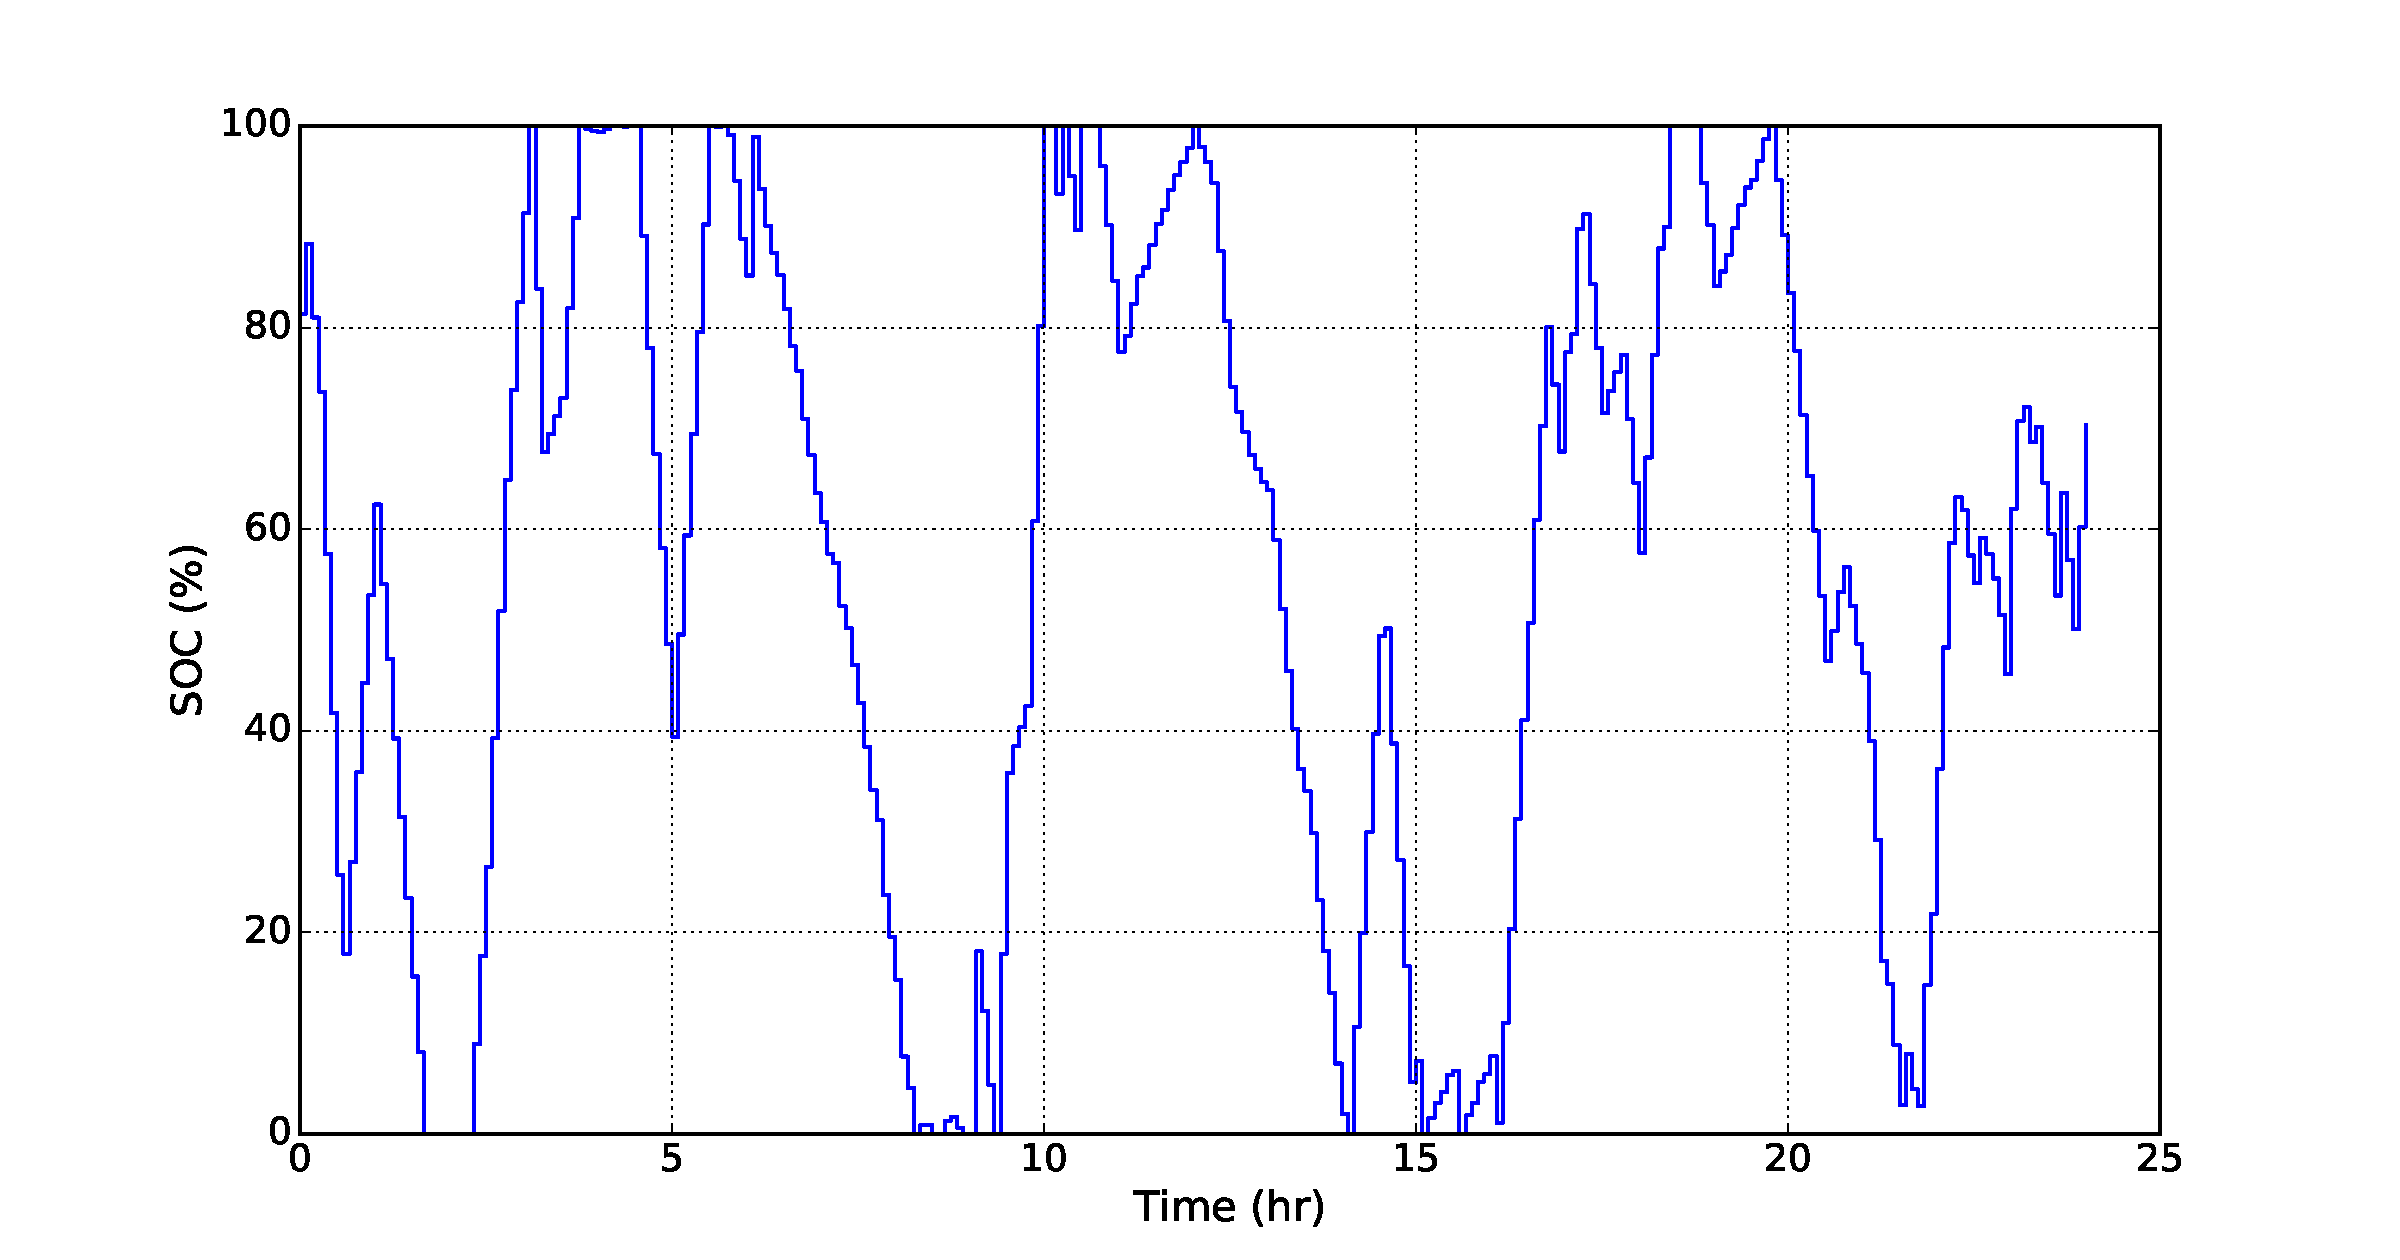
\includegraphics[width=\textwidth]{Figures/Plots/Simultaneous/SOC.pdf} \caption{State of charge of the battery}\label{socsim} \end{subfigure} \hfill
\begin{subfigure}[b]{0.49\textwidth} \includegraphics[width=\textwidth]{Figures/Plots/Simultaneous/P_band.pdf} \caption{Power of the battery with the regulation band}\label{pbandsim} \end{subfigure} \hfill
\caption{Battery performance obtained using simultaneous approach (shown only for day 91)}\label{perfsim}
\end{figure}
\begin{figure}[h!tp]
\centering
\begin{subfigure}[b]{0.49\textwidth} 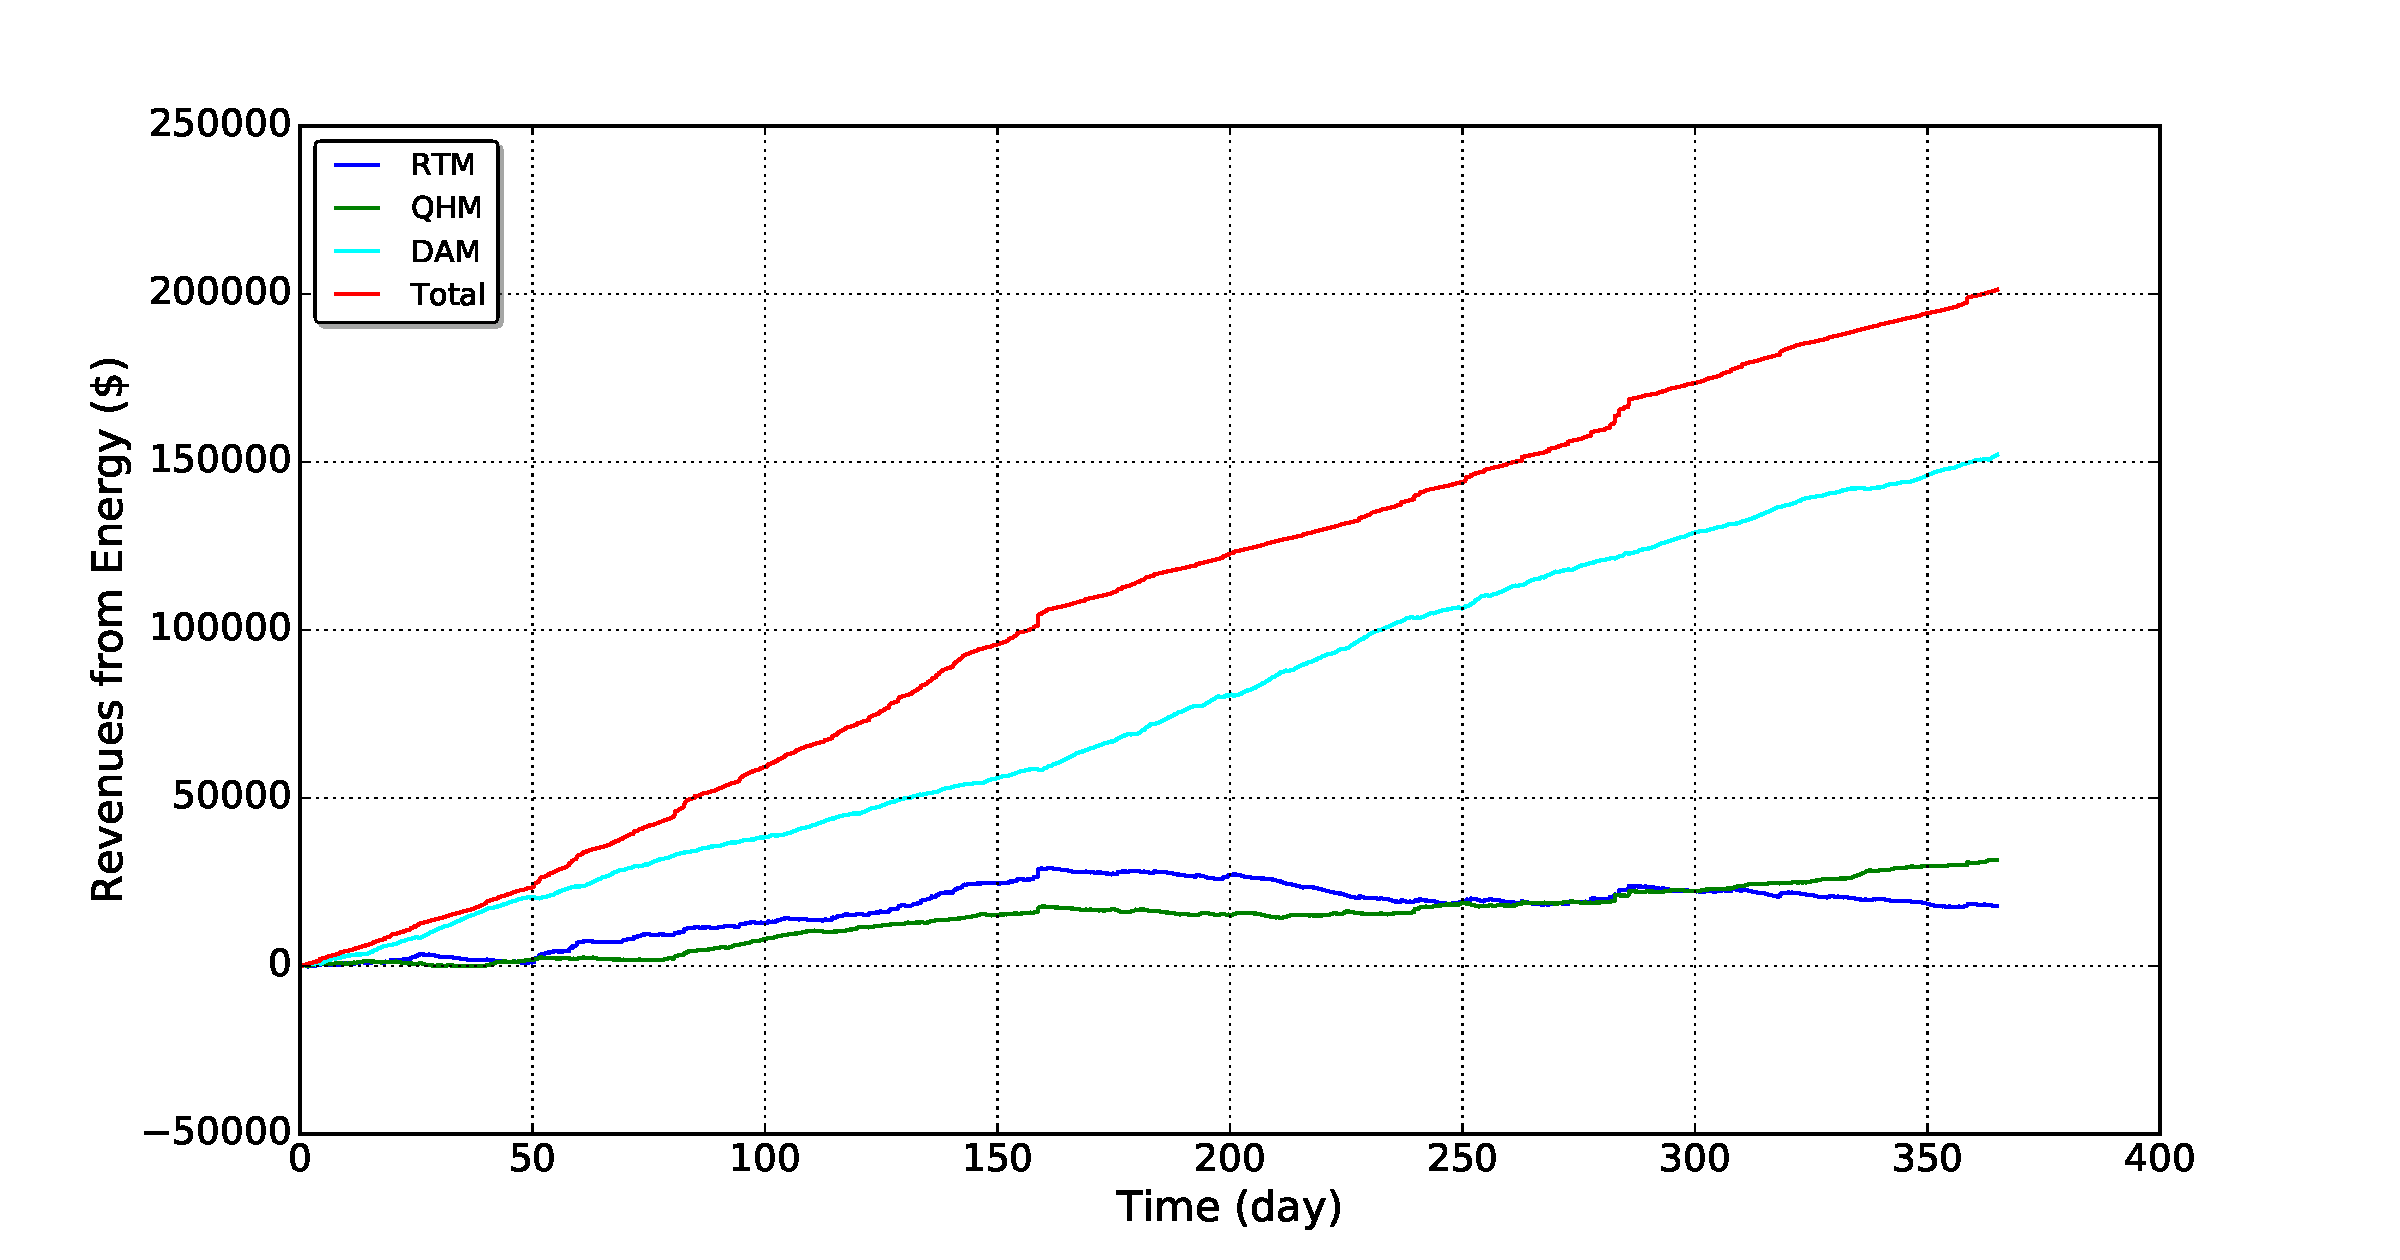
\includegraphics[width=\textwidth]{Figures/Plots/Simultaneous/E_Rev.pdf} \caption{Revenues from energy markets}\label{erevsim} \end{subfigure} \hfill
\begin{subfigure}[b]{0.49\textwidth} 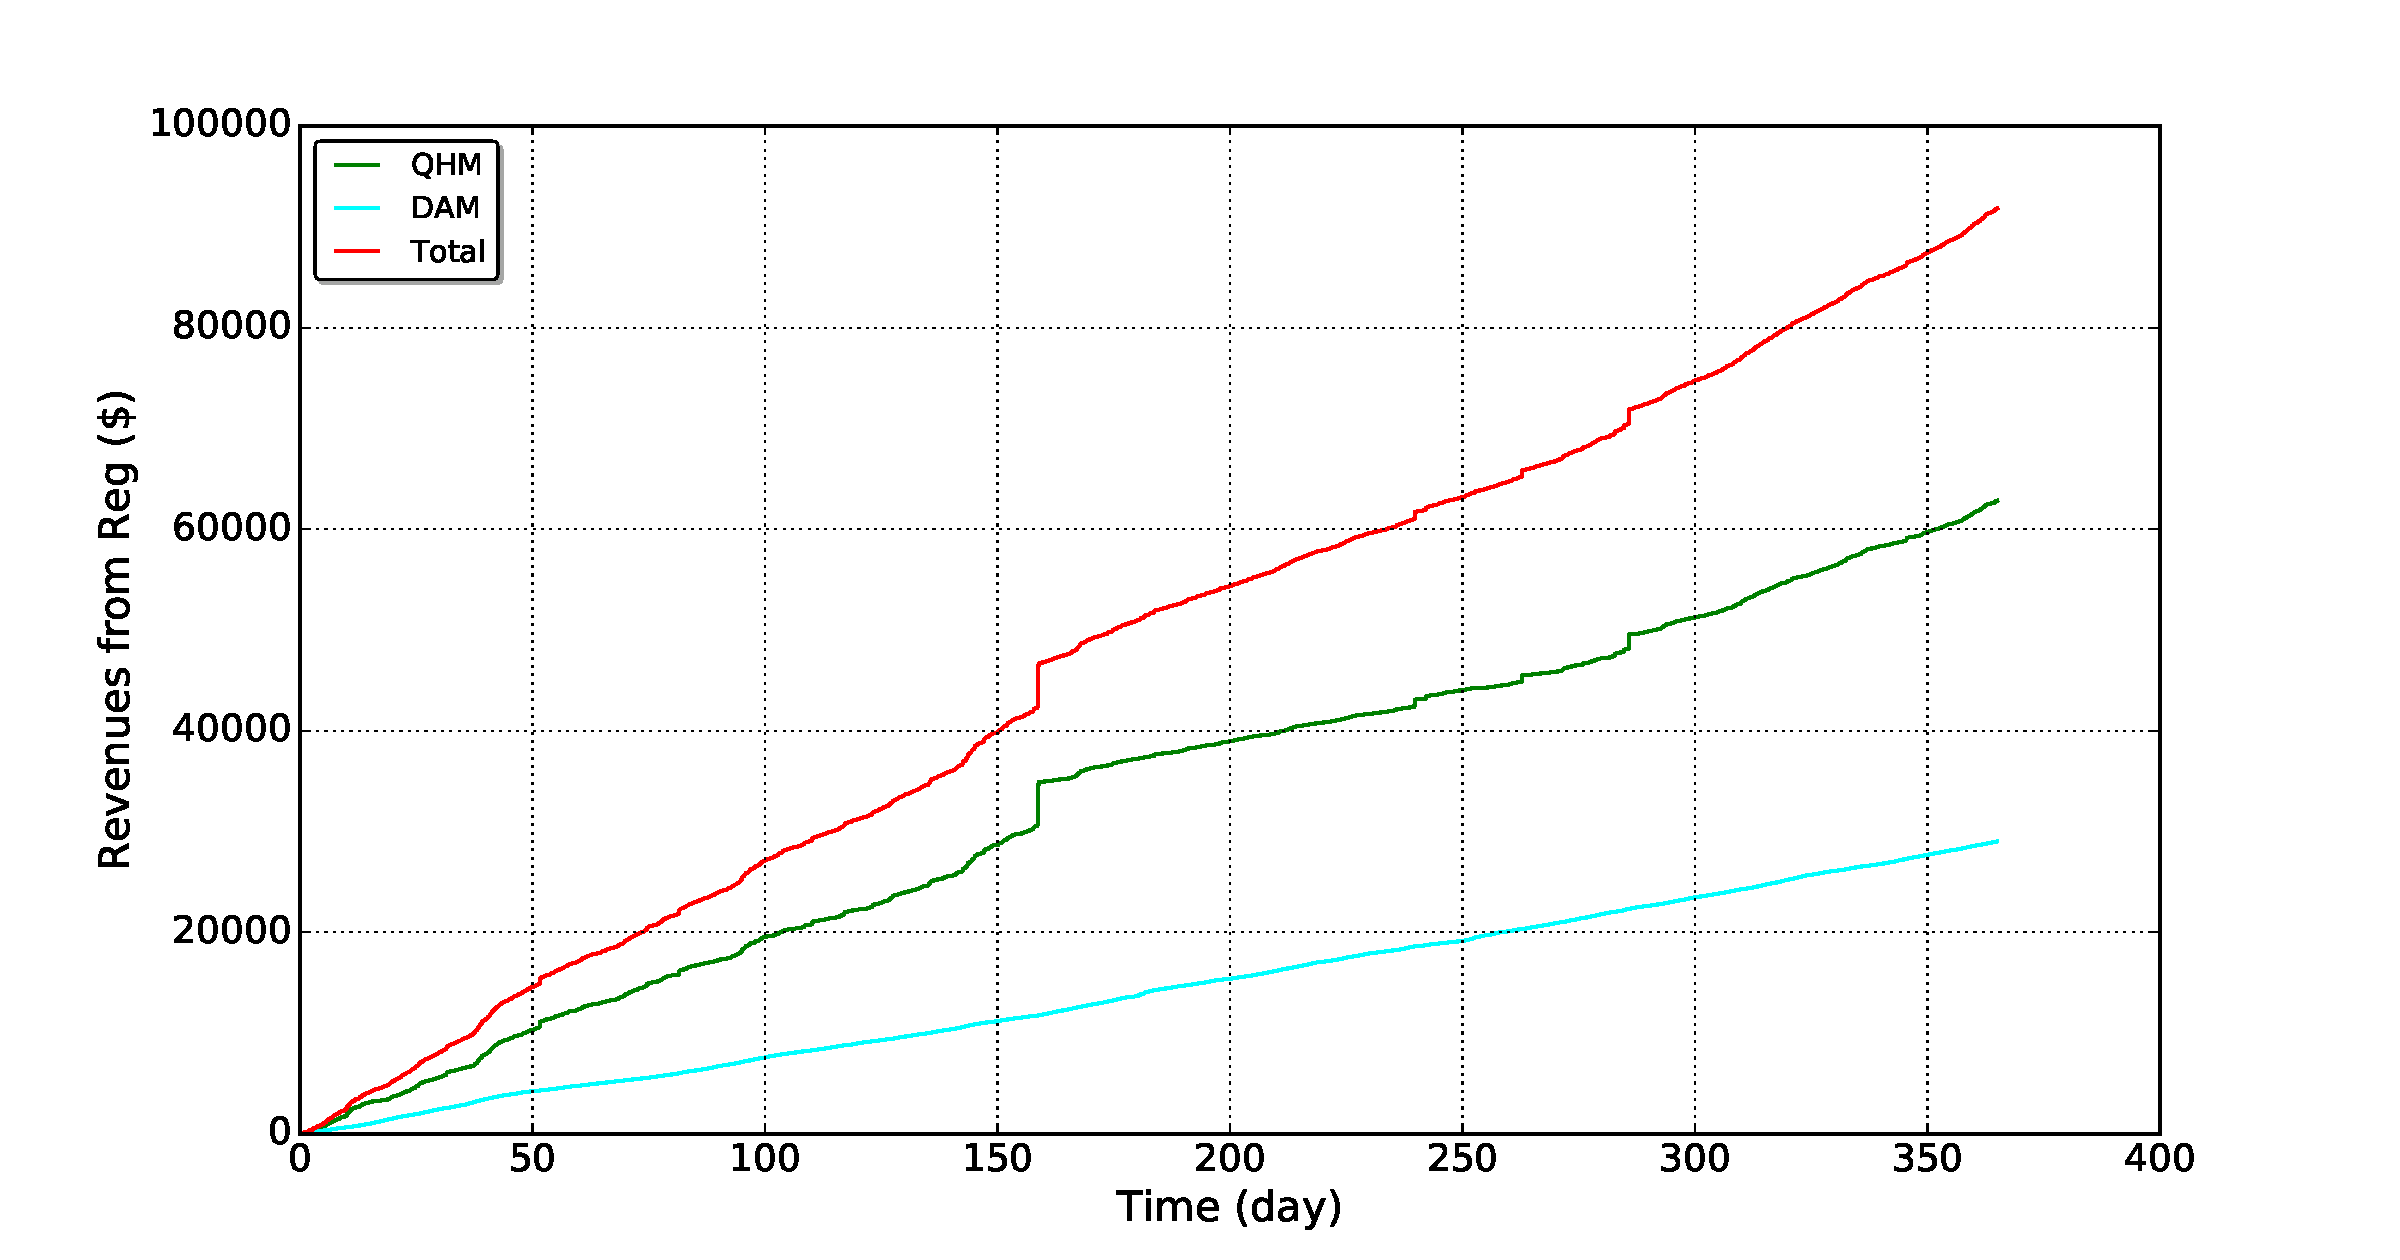
\includegraphics[width=\textwidth]{Figures/Plots/Simultaneous/Reg_Rev.pdf} \caption{Revenues from regulation markets}\label{regrevsim} \end{subfigure} \hfill
\begin{subfigure}[b]{0.49\textwidth} 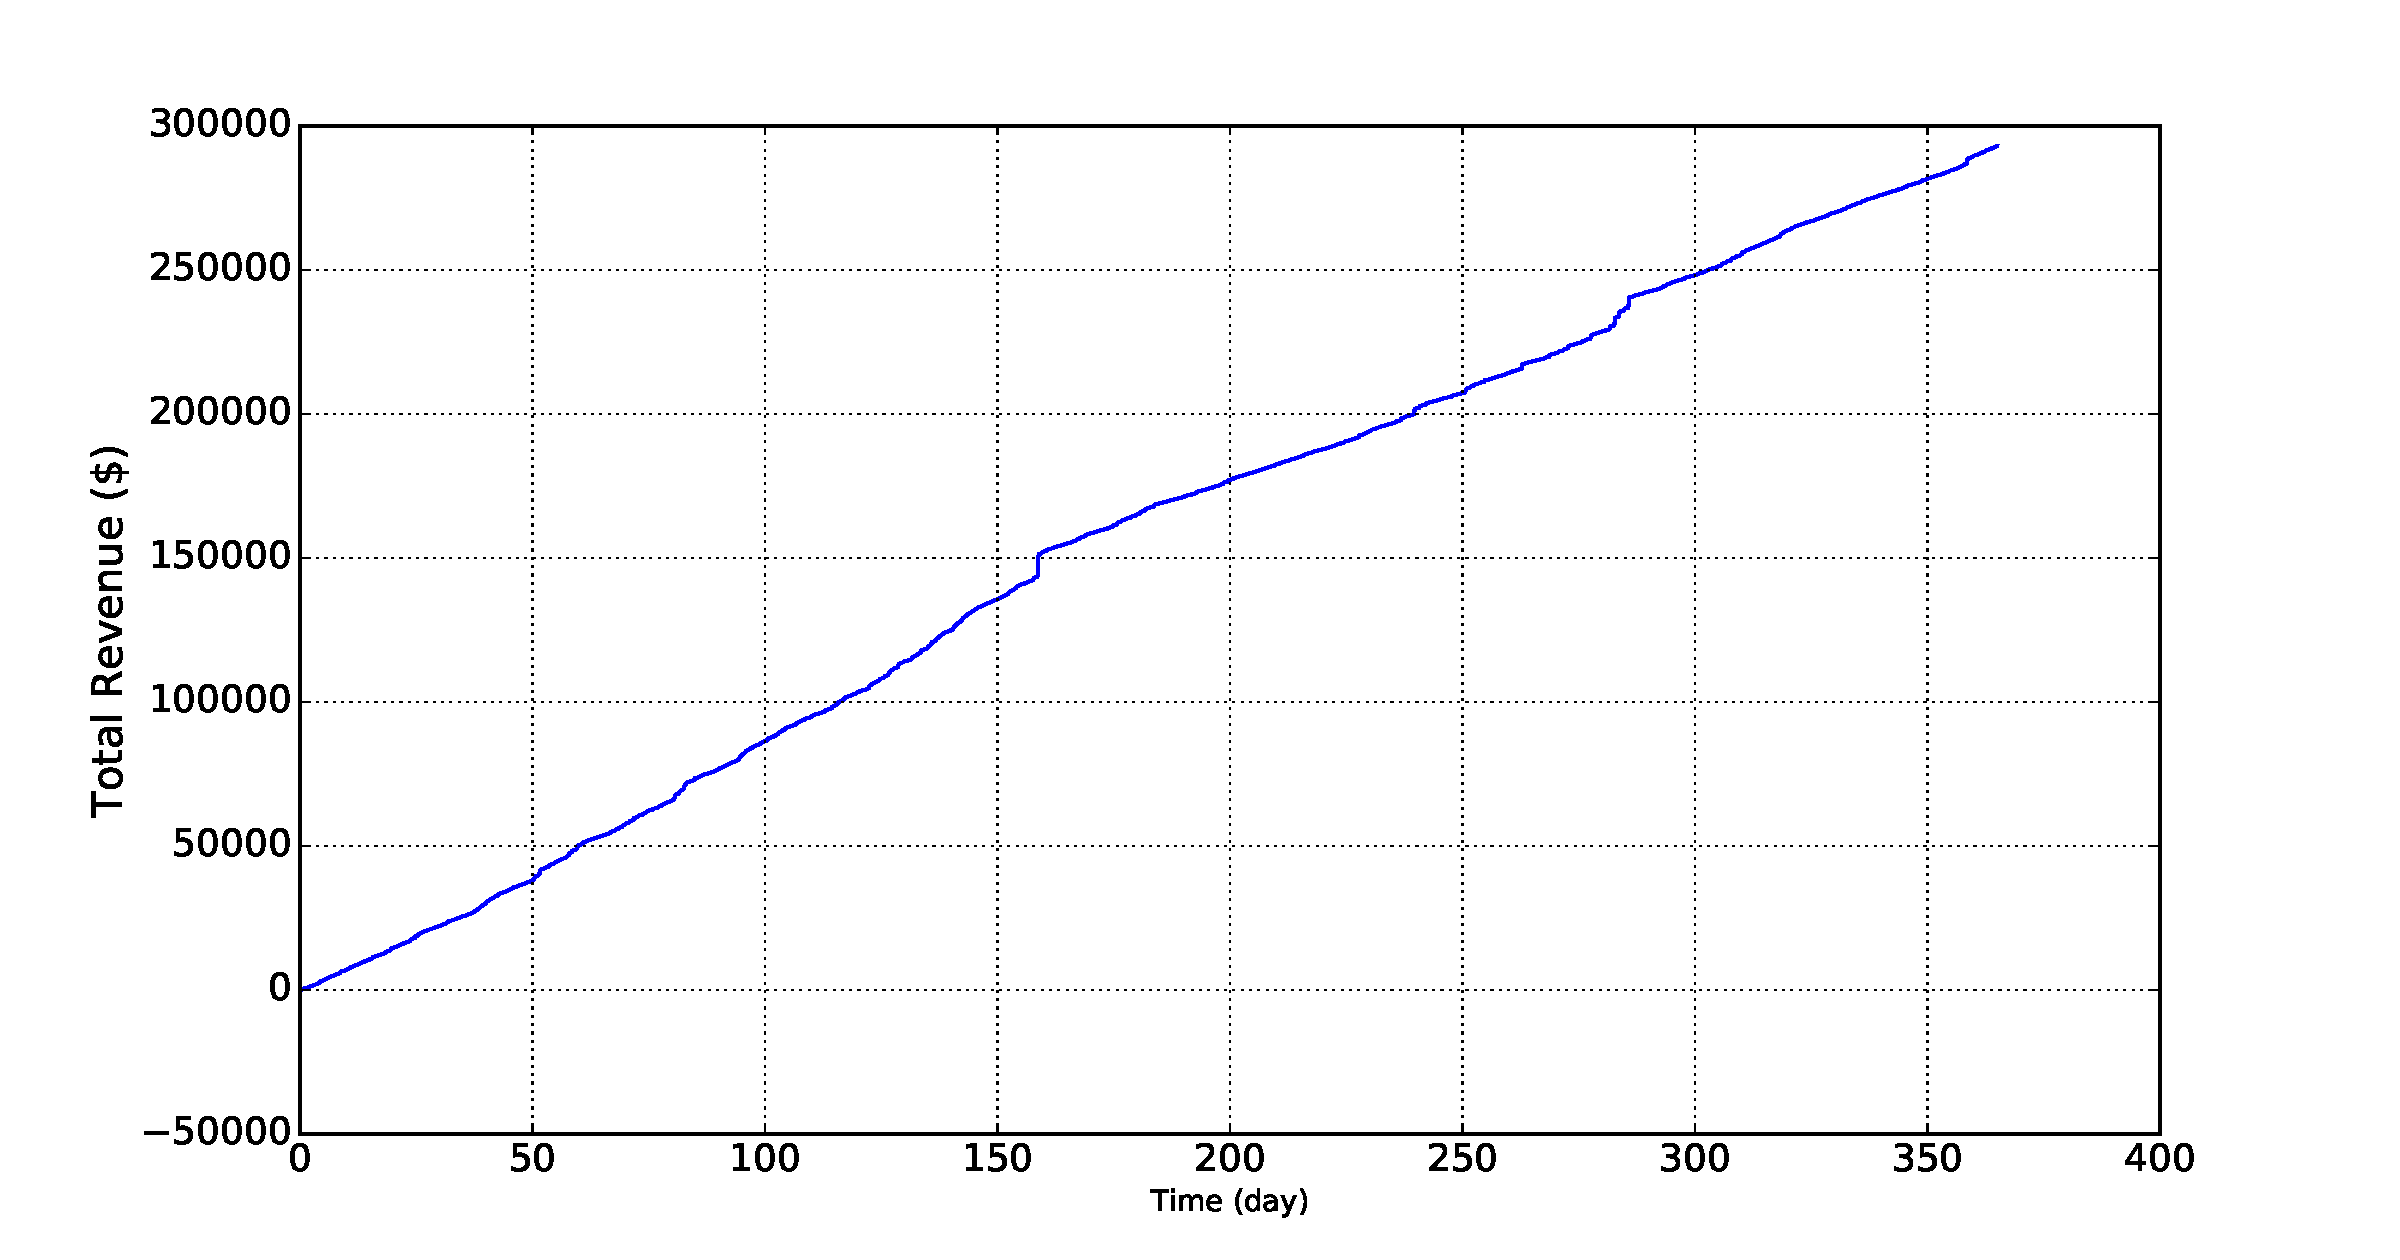
\includegraphics[width=\textwidth]{Figures/Plots/Simultaneous/Tot_Rev.pdf} \caption{Total revenues}\label{totrevsim}\end{subfigure} \hfill
\caption{Revenues obtained using simultaneous approach (shown only for day 91)}\label{revsim}
\end{figure}

\subsection{Rolling (1 day) horizon approach}
The problem was formulated in Julia programming language with JuMP modeling language and was solved with Gurobi solver. The problem for each day is a linear program whose size is as follows:
\begin{itemize}
\item 3,025 variables each day
\item 2,497 linear constraints each day
\end{itemize}
The computation time to solve the problem was slightly between 0.01 and 0.02 second and about 5-10 seconds to solve the problem sequentially day-by-day for the whole year.

The optimal revenues obtained with this approach were as follows:
\begin{itemize}
\item Total annual revenues: \$296,985
\item Revenues from energy sale: \$205,835
\item Revenues from regulation: \$91,150.
\end{itemize}

The optimal battery power to the power grid, the optimum regulation up and down capacities, the optimum battery performance curves and the revenue profiles during one of the days (day 91) in the year have been shown in Figures \ref{phor}, \ref{reghor}, \ref{perfhor} and \ref{revhor} respectively.
\begin{figure}[h!tp]
\centering
\begin{subfigure}[b]{0.49\textwidth} 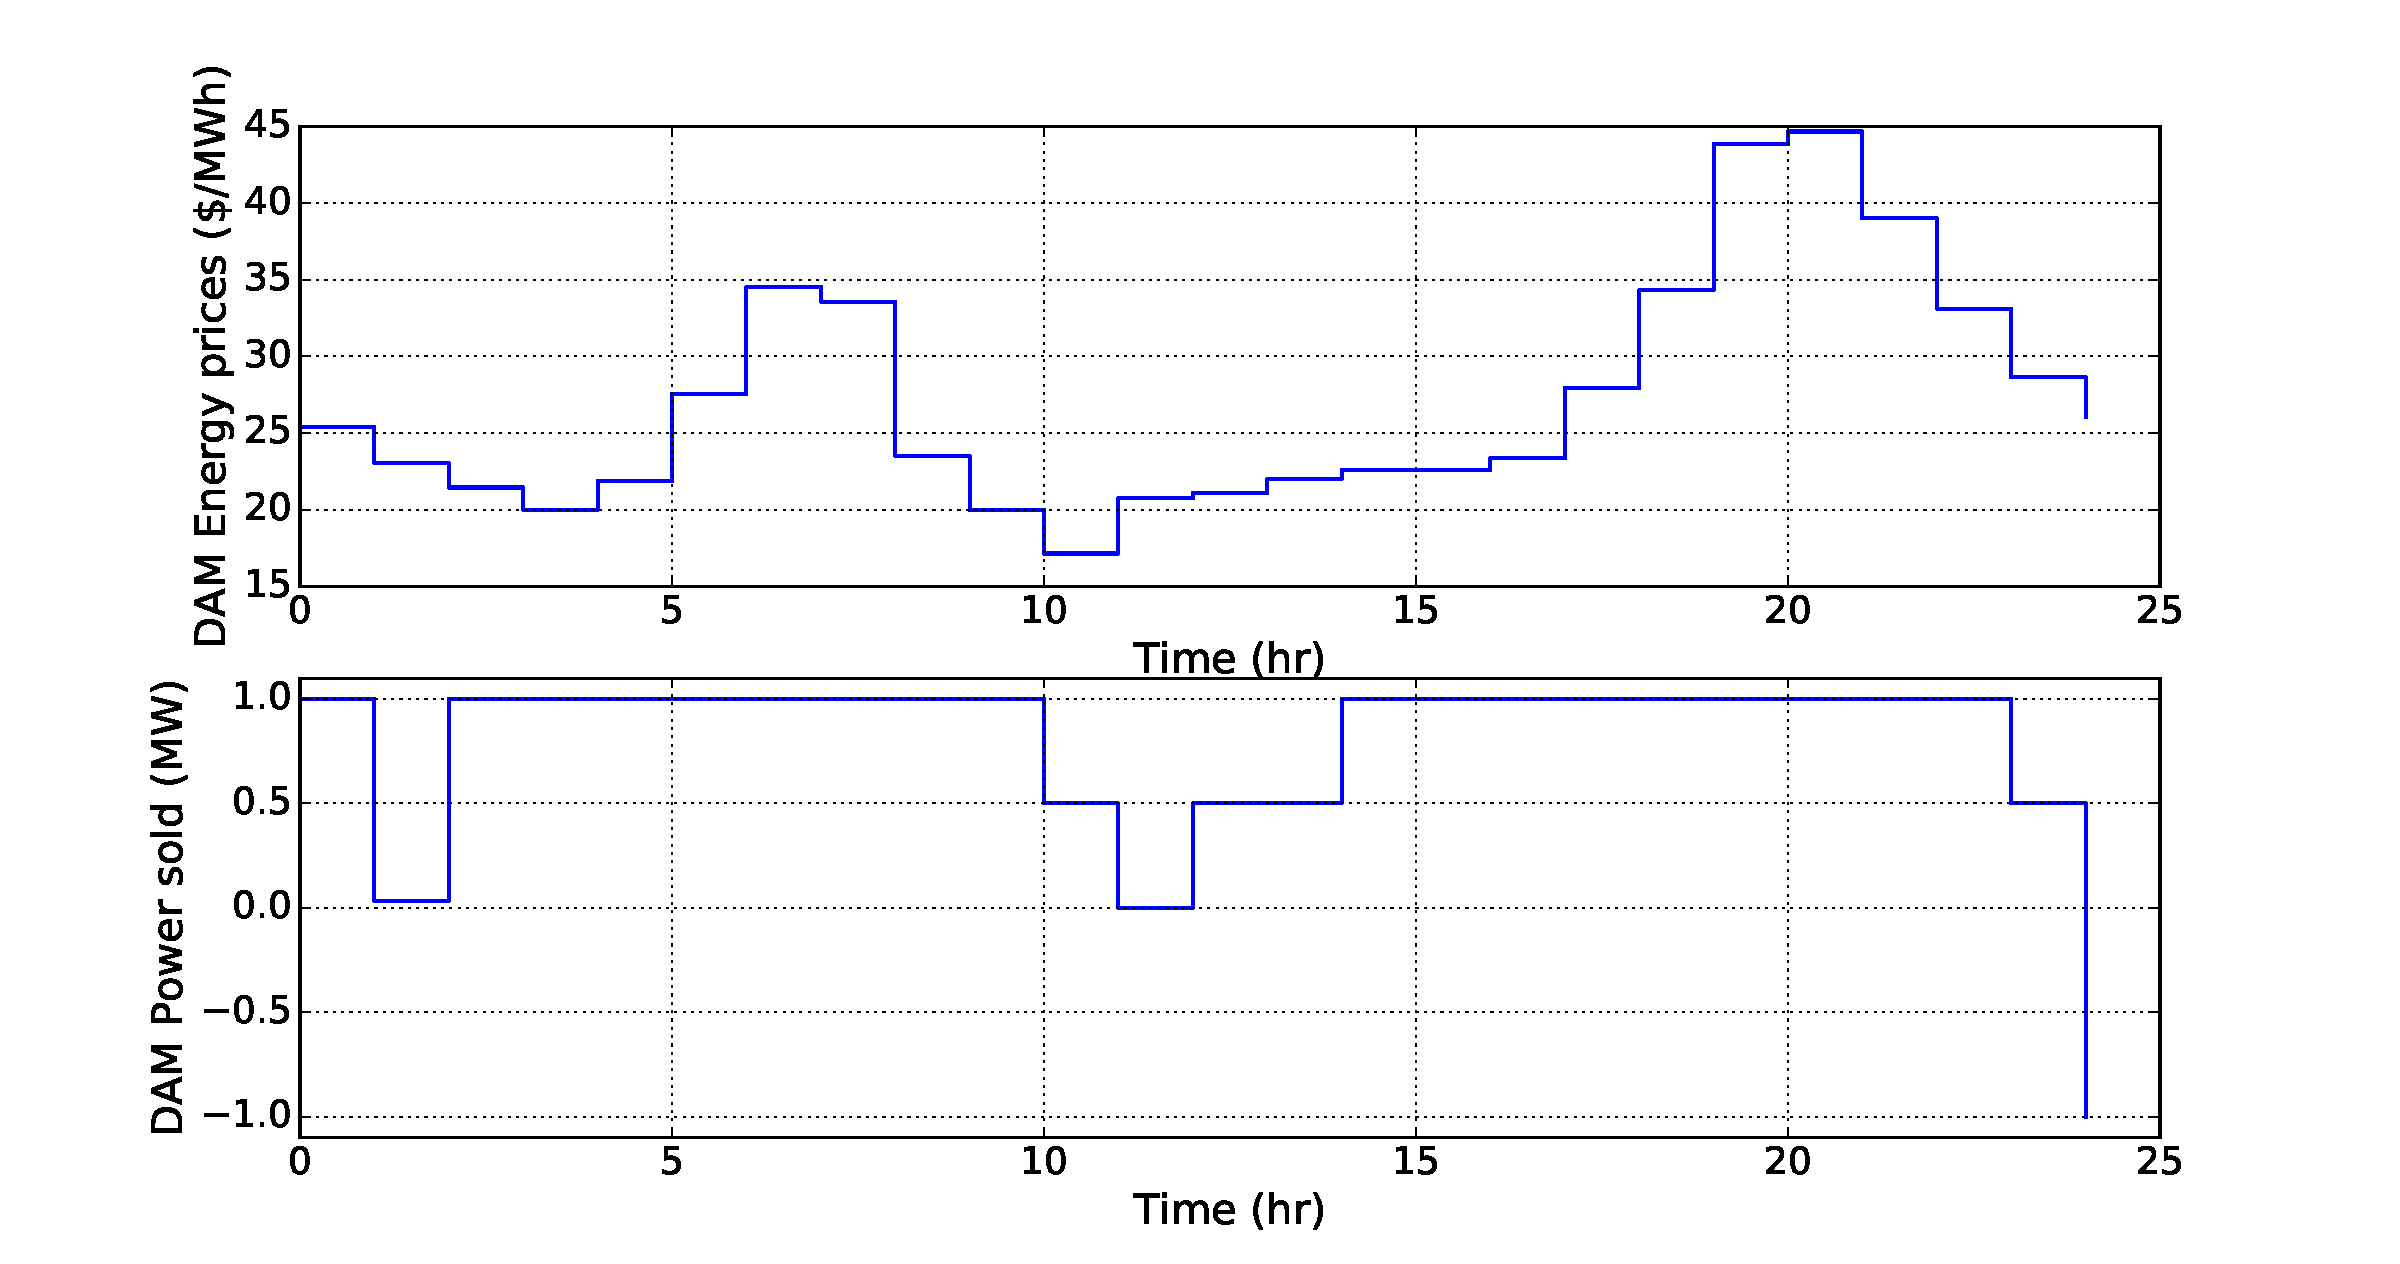
\includegraphics[width=\textwidth]{Figures/Plots/Horizon/DAM_P.pdf} \caption{Day-ahead market}\label{damphor} \end{subfigure} \hfill
\begin{subfigure}[b]{0.49\textwidth} 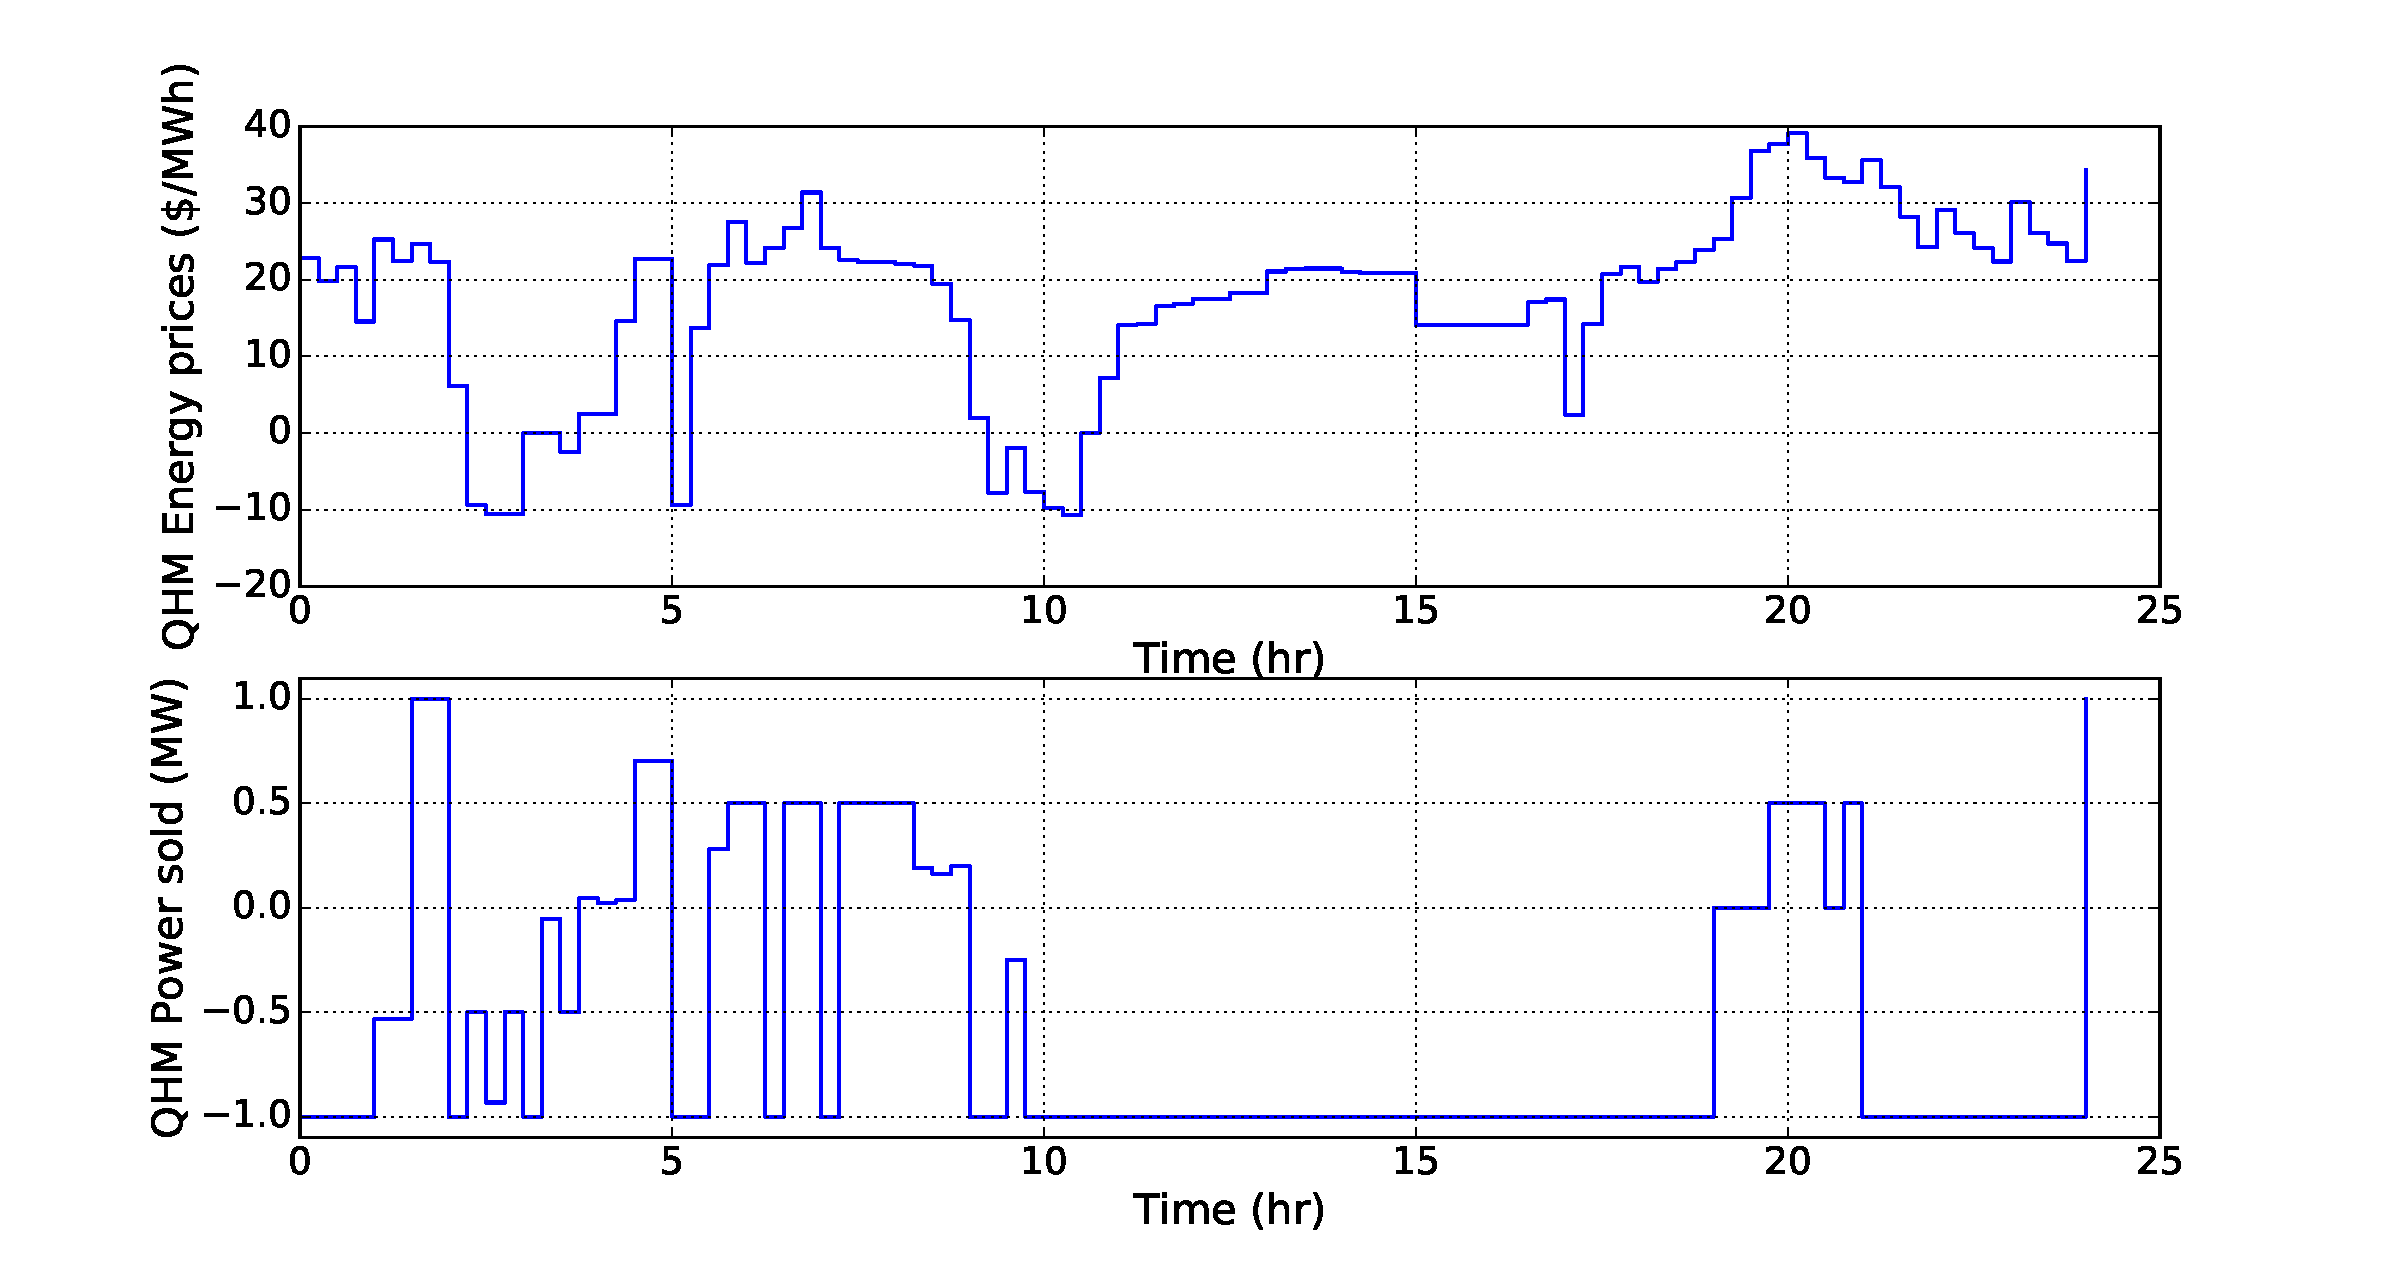
\includegraphics[width=\textwidth]{Figures/Plots/Horizon/QHM_P.pdf} \caption{Quarter-hourly market}\label{qhmphor} \end{subfigure} \hfill
\begin{subfigure}[b]{0.49\textwidth} 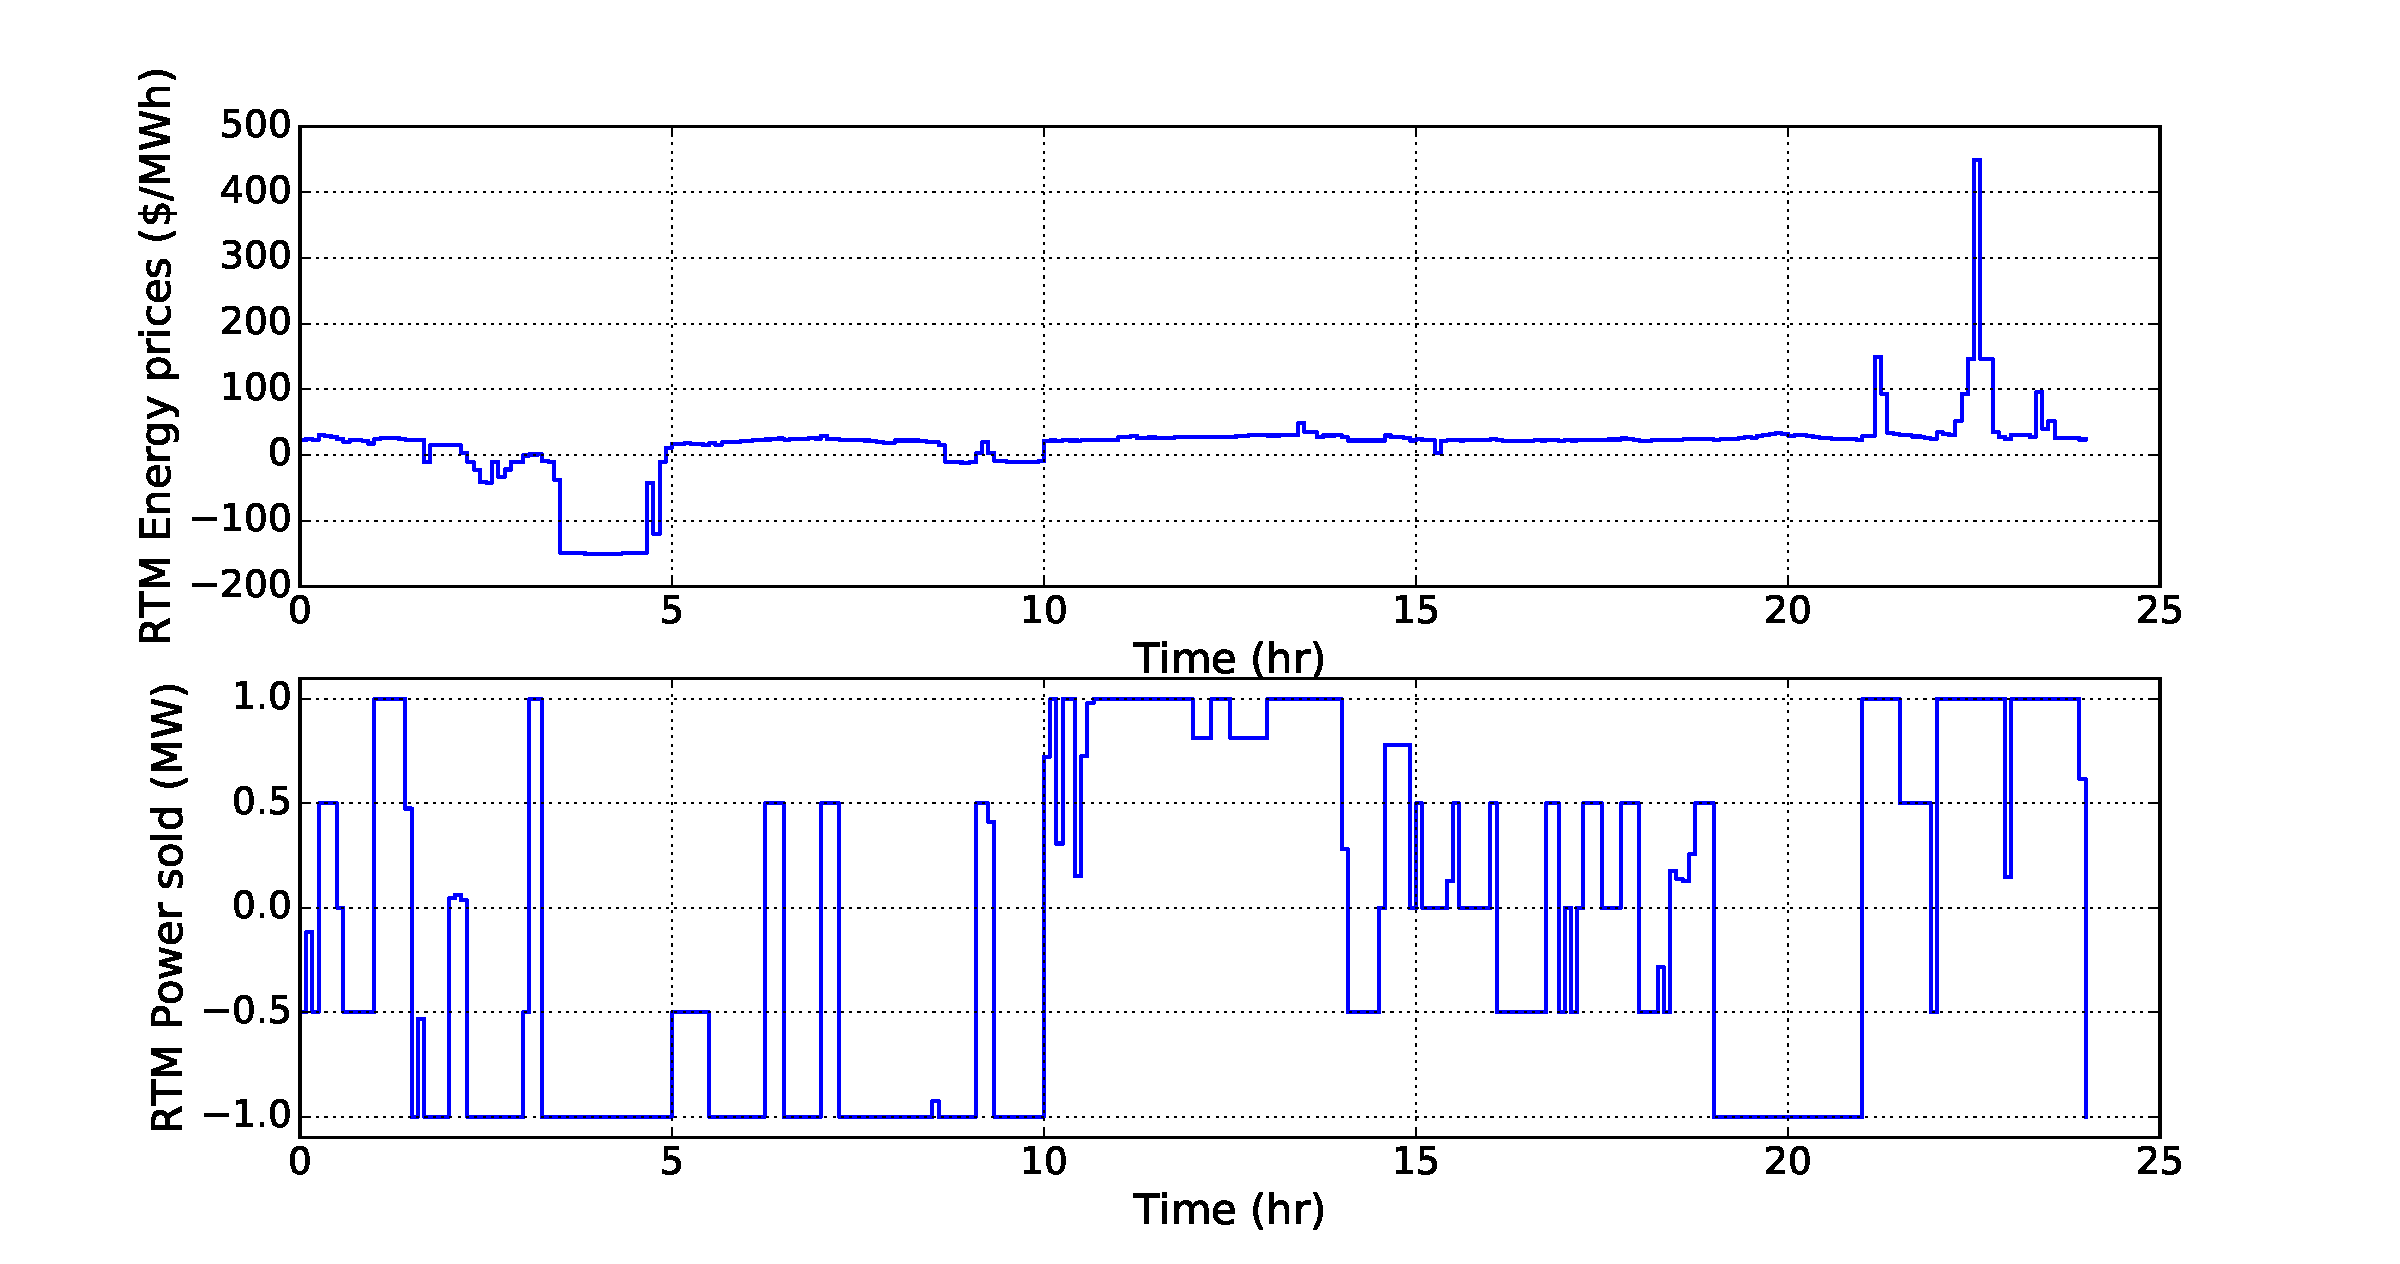
\includegraphics[width=\textwidth]{Figures/Plots/Horizon/RTM_P.pdf} \caption{Real-time market}\label{rtmphor}\end{subfigure} \hfill
\caption{Optimal power obtained using rolling horizon approach (shown only for day 91)}\label{phor}
\end{figure}
\begin{figure}[h!tp]
\centering
\begin{subfigure}[b]{0.49\textwidth} \includegraphics[width=\textwidth]{Figures/Plots/Horizon/DAM_Reg.pdf} \caption{Day-ahead market}\label{damreghor} \end{subfigure} \hfill
\begin{subfigure}[b]{0.49\textwidth} \includegraphics[width=\textwidth]{Figures/Plots/Horizon/QHM_Reg.pdf} \caption{Quarter-hourly market}\label{qhmreghor} \end{subfigure} \hfill
\caption{Optimal regulation capacities obtained using rolling horizon approach (shown only for day 91)}\label{reghor}
\end{figure}
\begin{figure}[h!tp]
\centering
\begin{subfigure}[b]{0.49\textwidth} 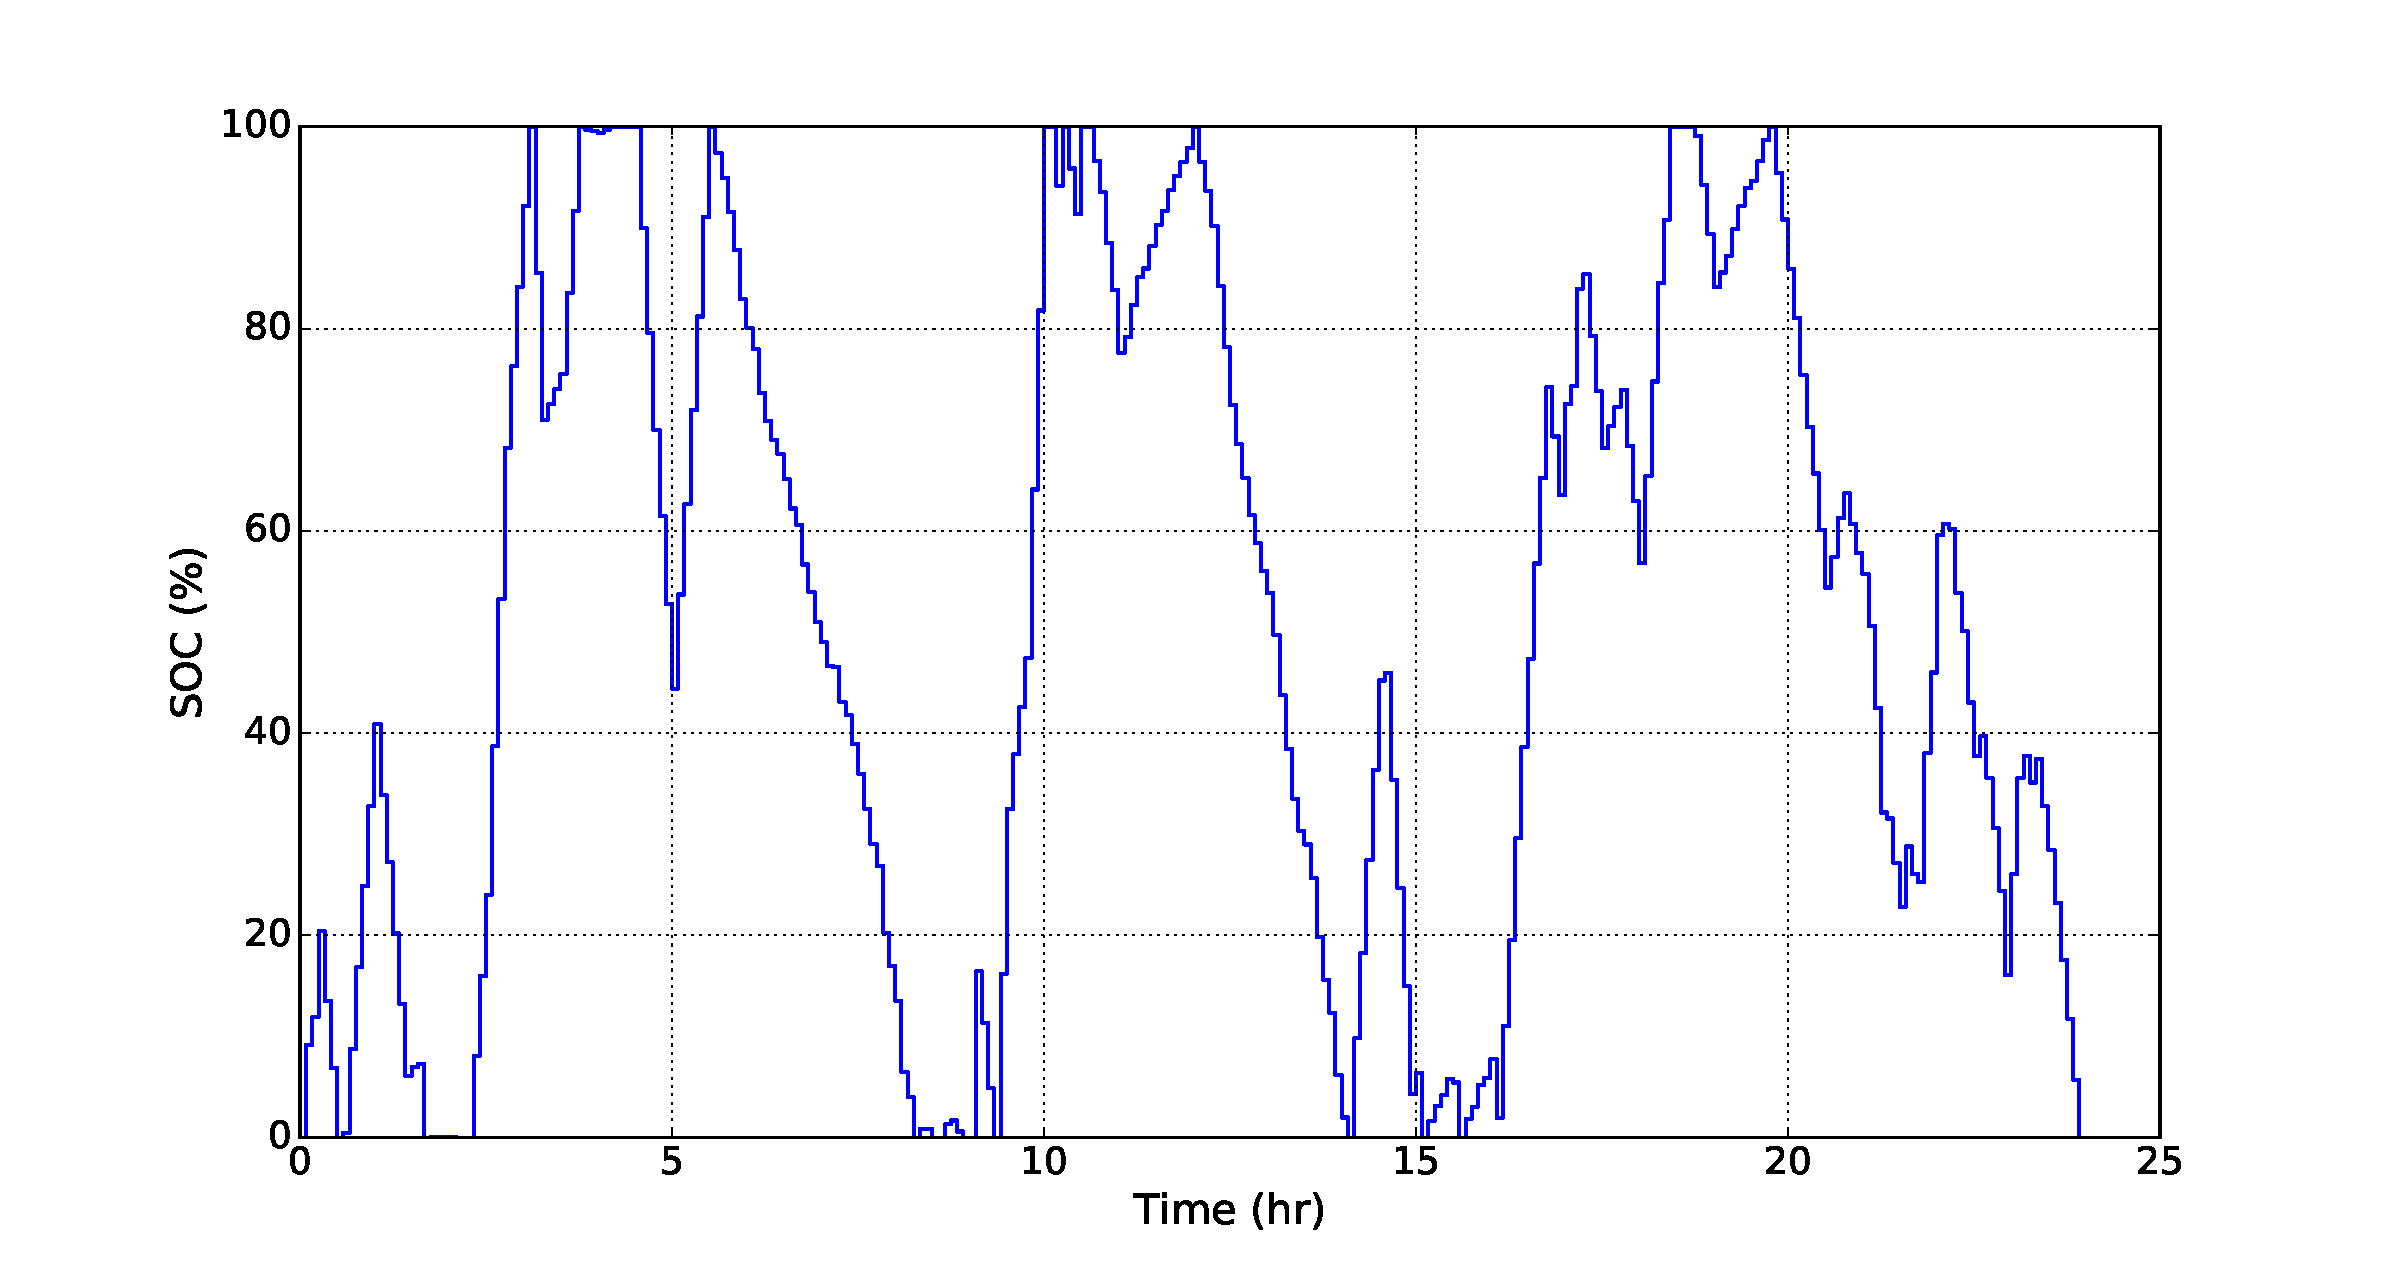
\includegraphics[width=\textwidth]{Figures/Plots/Horizon/SOC.pdf} \caption{State of charge of the battery}\label{sochor} \end{subfigure} \hfill
\begin{subfigure}[b]{0.49\textwidth} \includegraphics[width=\textwidth]{Figures/Plots/Horizon/P_band.pdf} \caption{Power of the battery with the regulation band}\label{pbandhor} \end{subfigure} \hfill
\caption{Battery performance obtained using rolling horizon approach (shown only for day 91)}\label{perfhor}
\end{figure}
\begin{figure}[h!tp]
\centering
\begin{subfigure}[b]{0.49\textwidth} 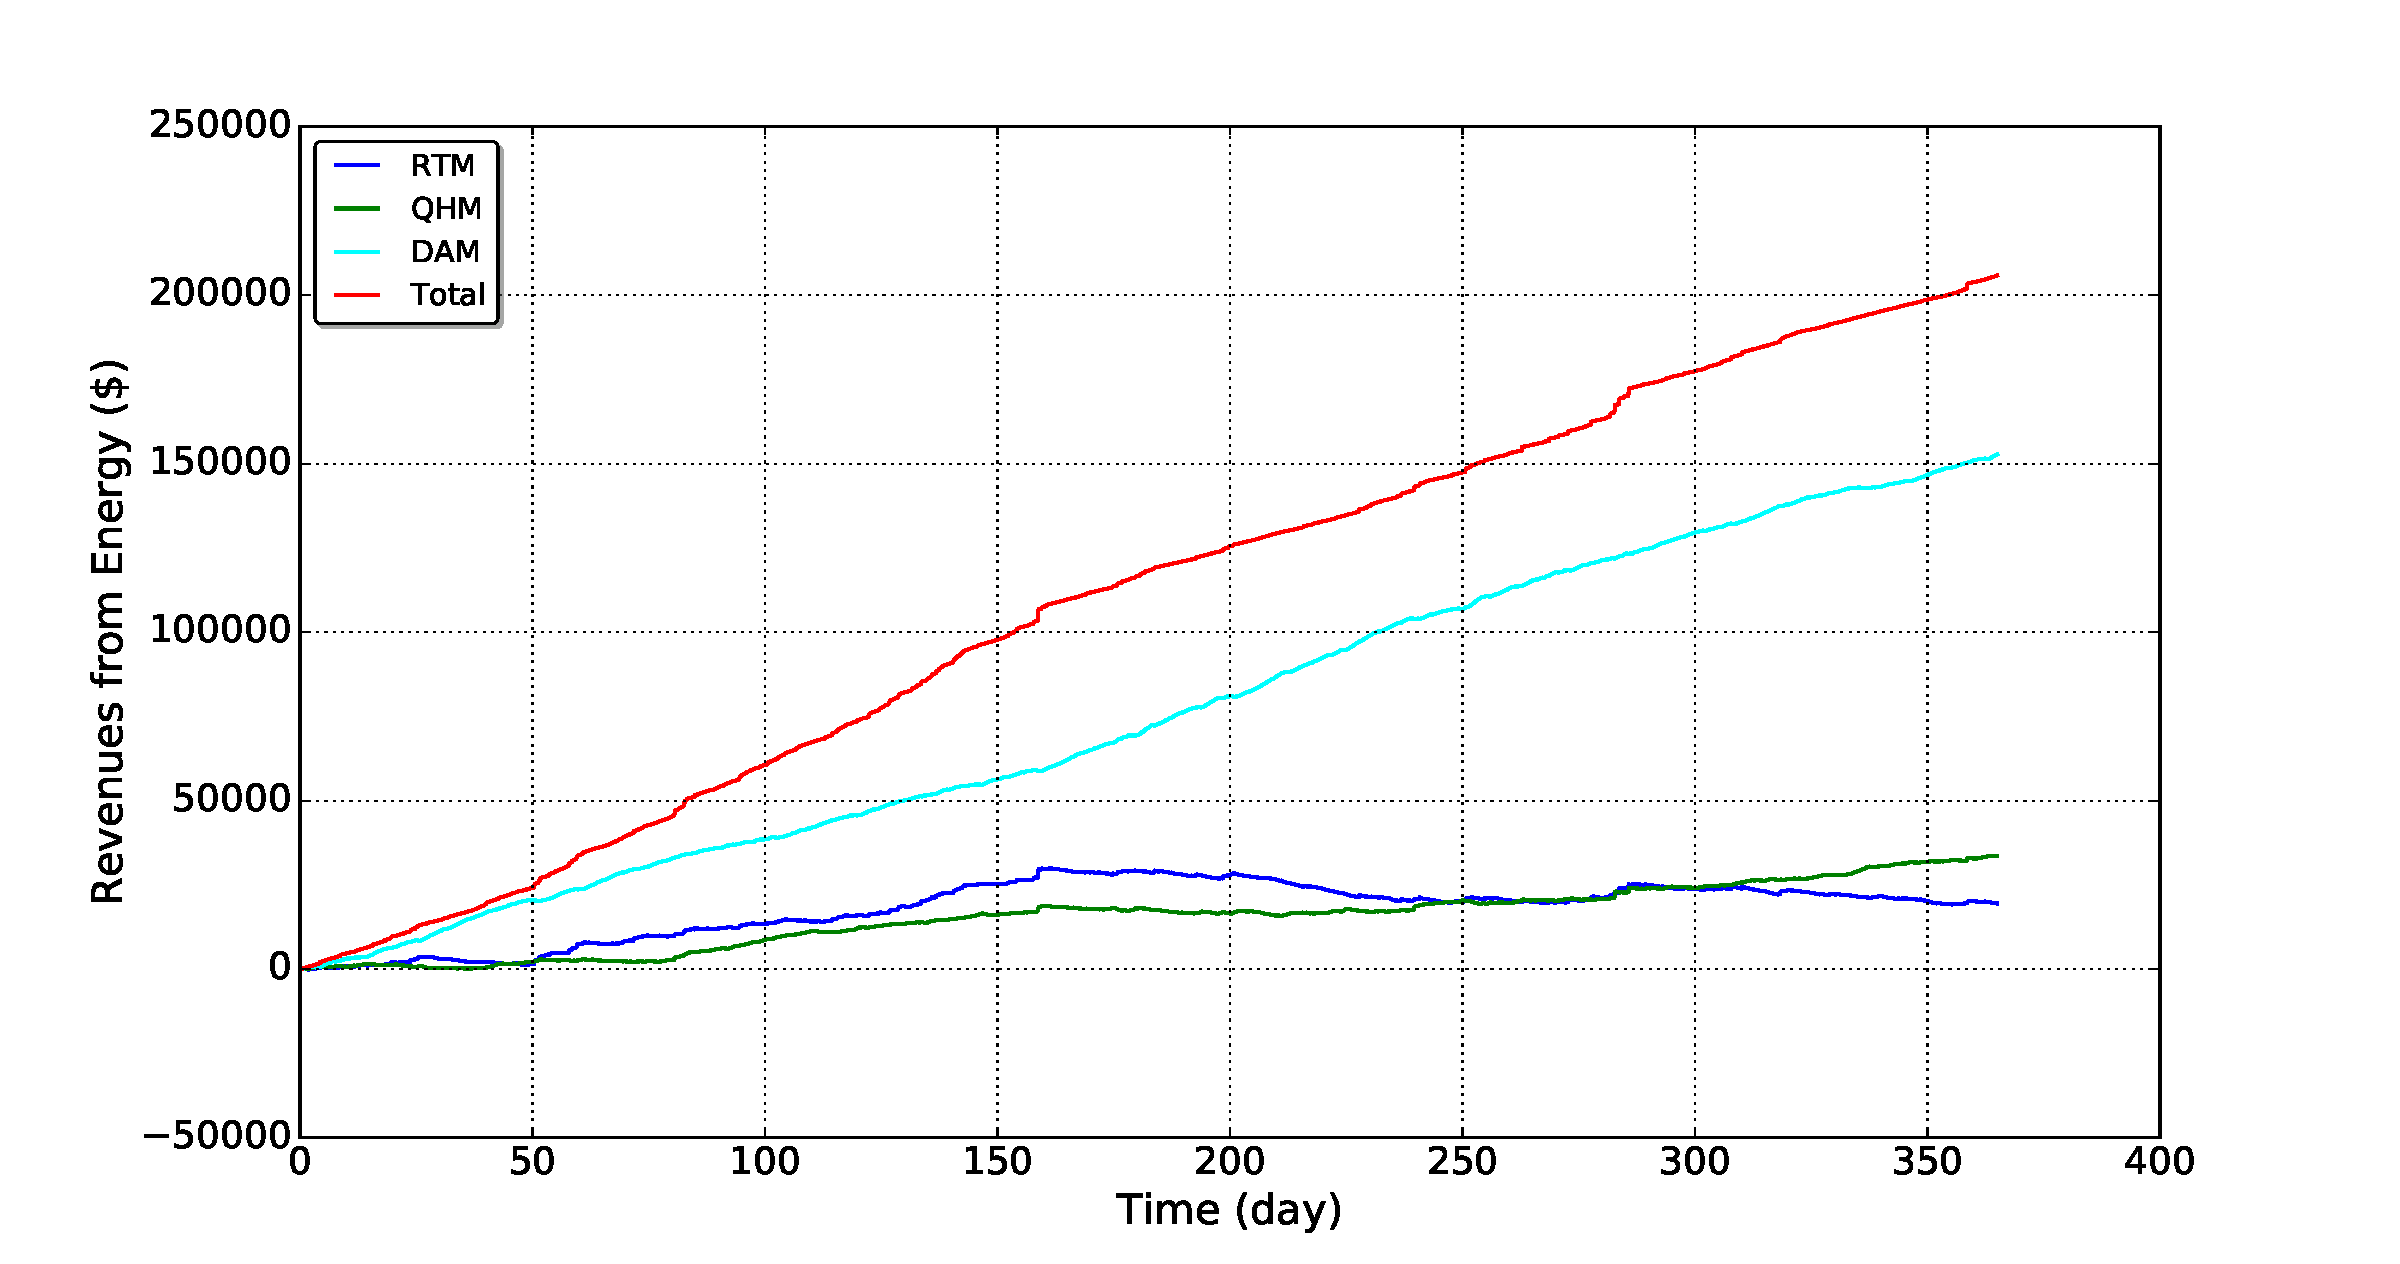
\includegraphics[width=\textwidth]{Figures/Plots/Horizon/Rev_E.pdf} \caption{Revenues from energy markets}\label{erevhor} \end{subfigure} \hfill
\begin{subfigure}[b]{0.49\textwidth} 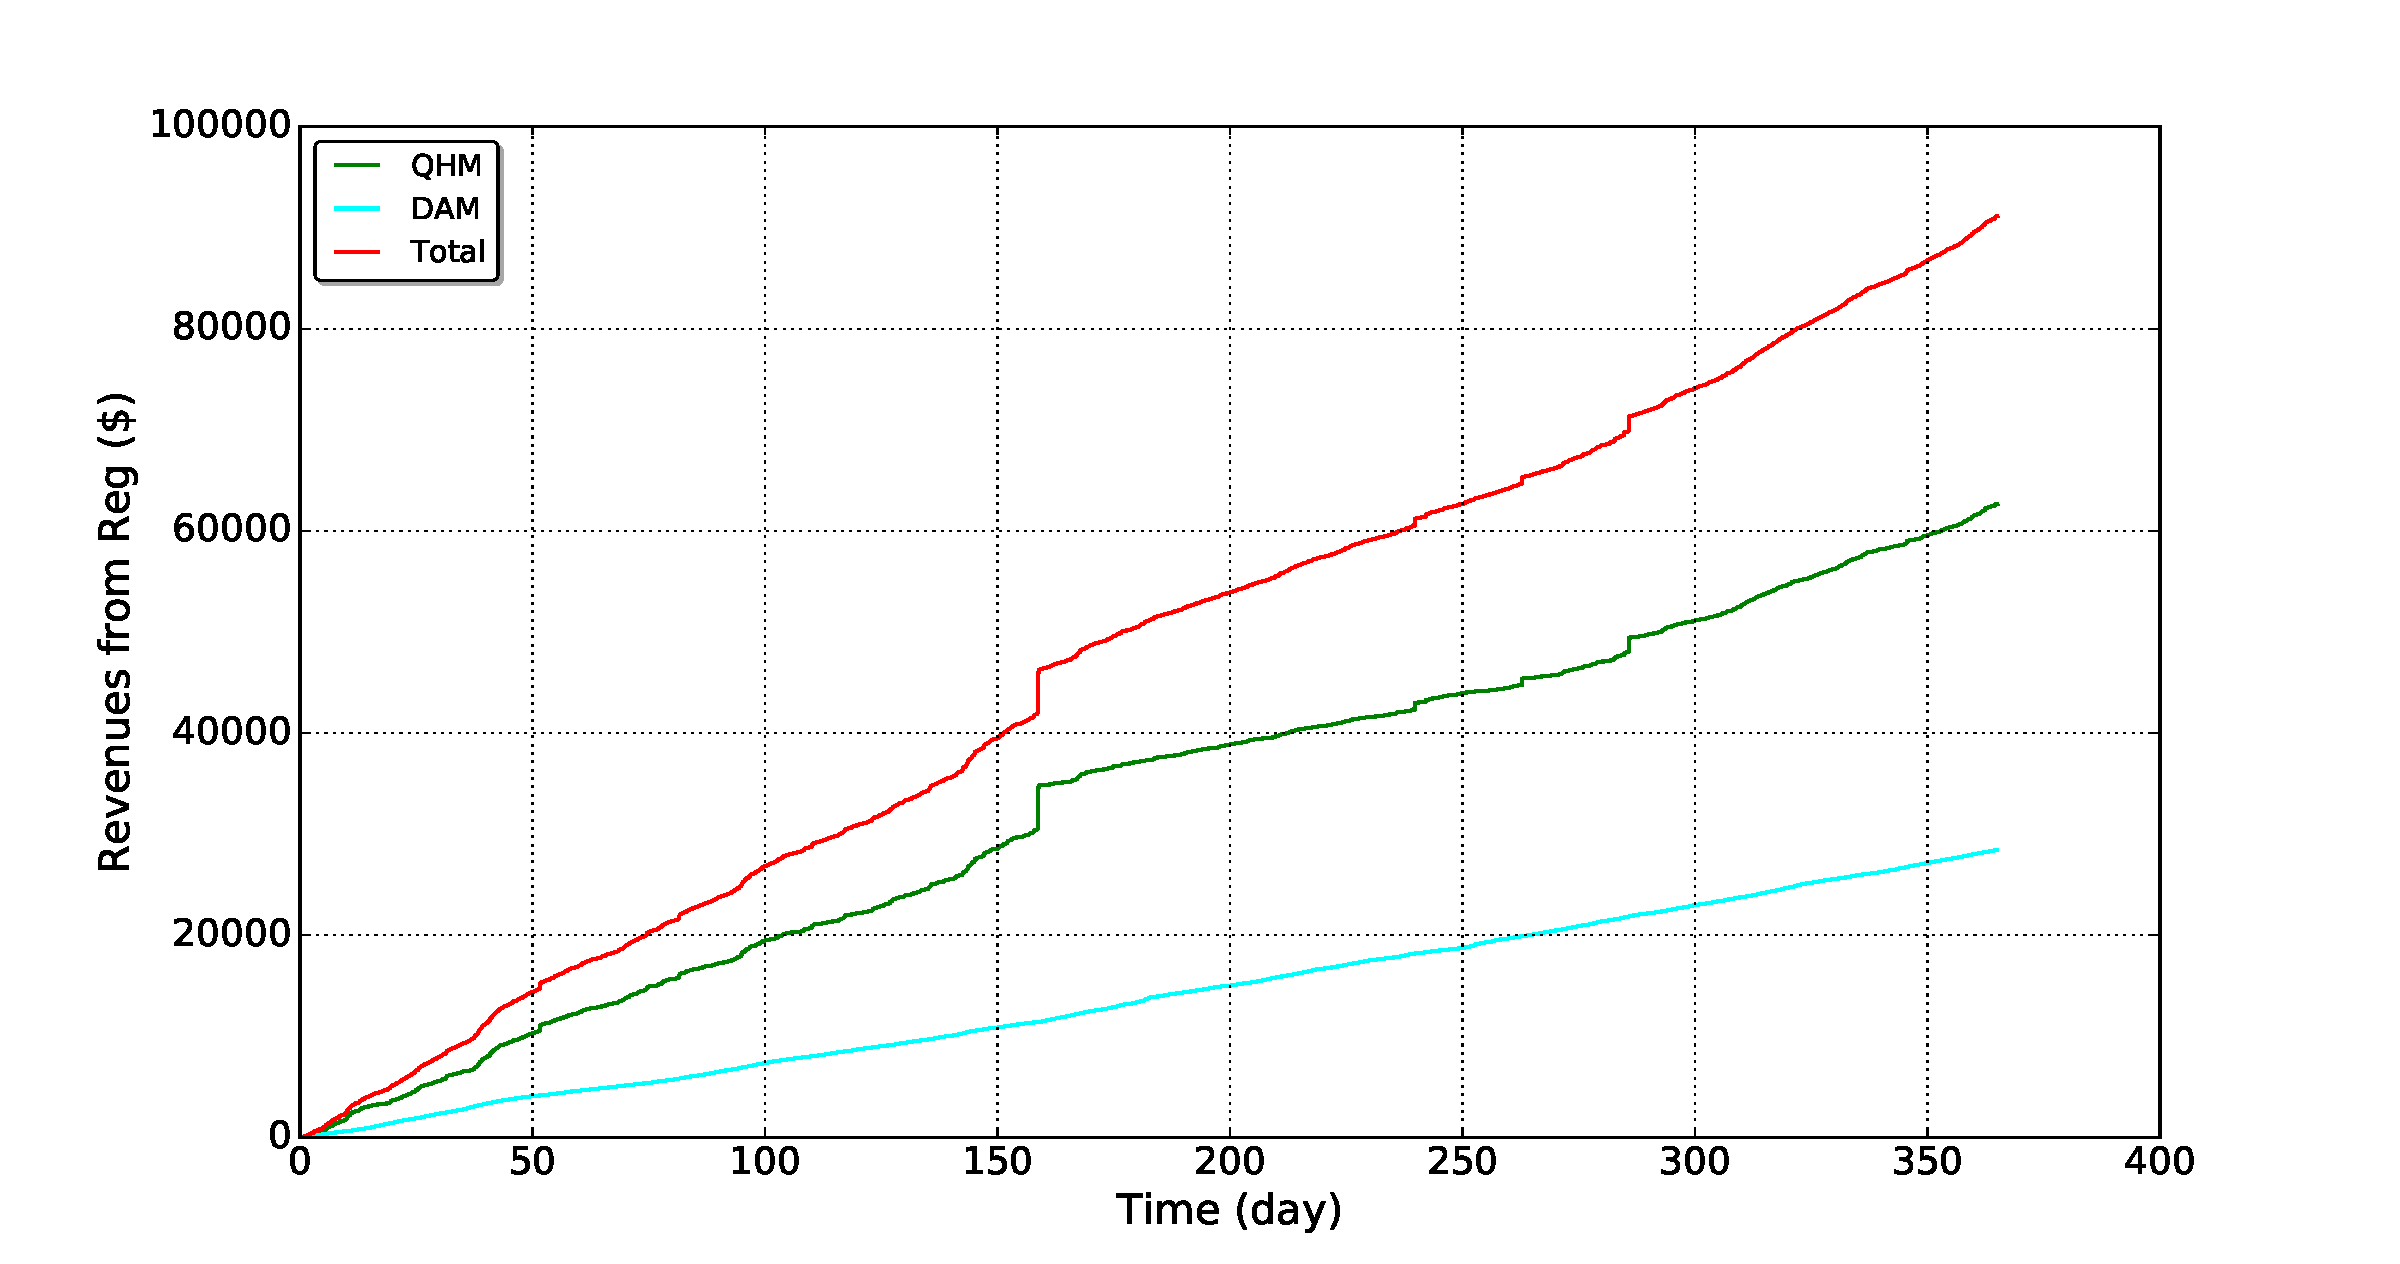
\includegraphics[width=\textwidth]{Figures/Plots/Horizon/Rev_Reg.pdf} \caption{Revenues from regulation markets}\label{regrevhor} \end{subfigure} \hfill
\begin{subfigure}[b]{0.49\textwidth} 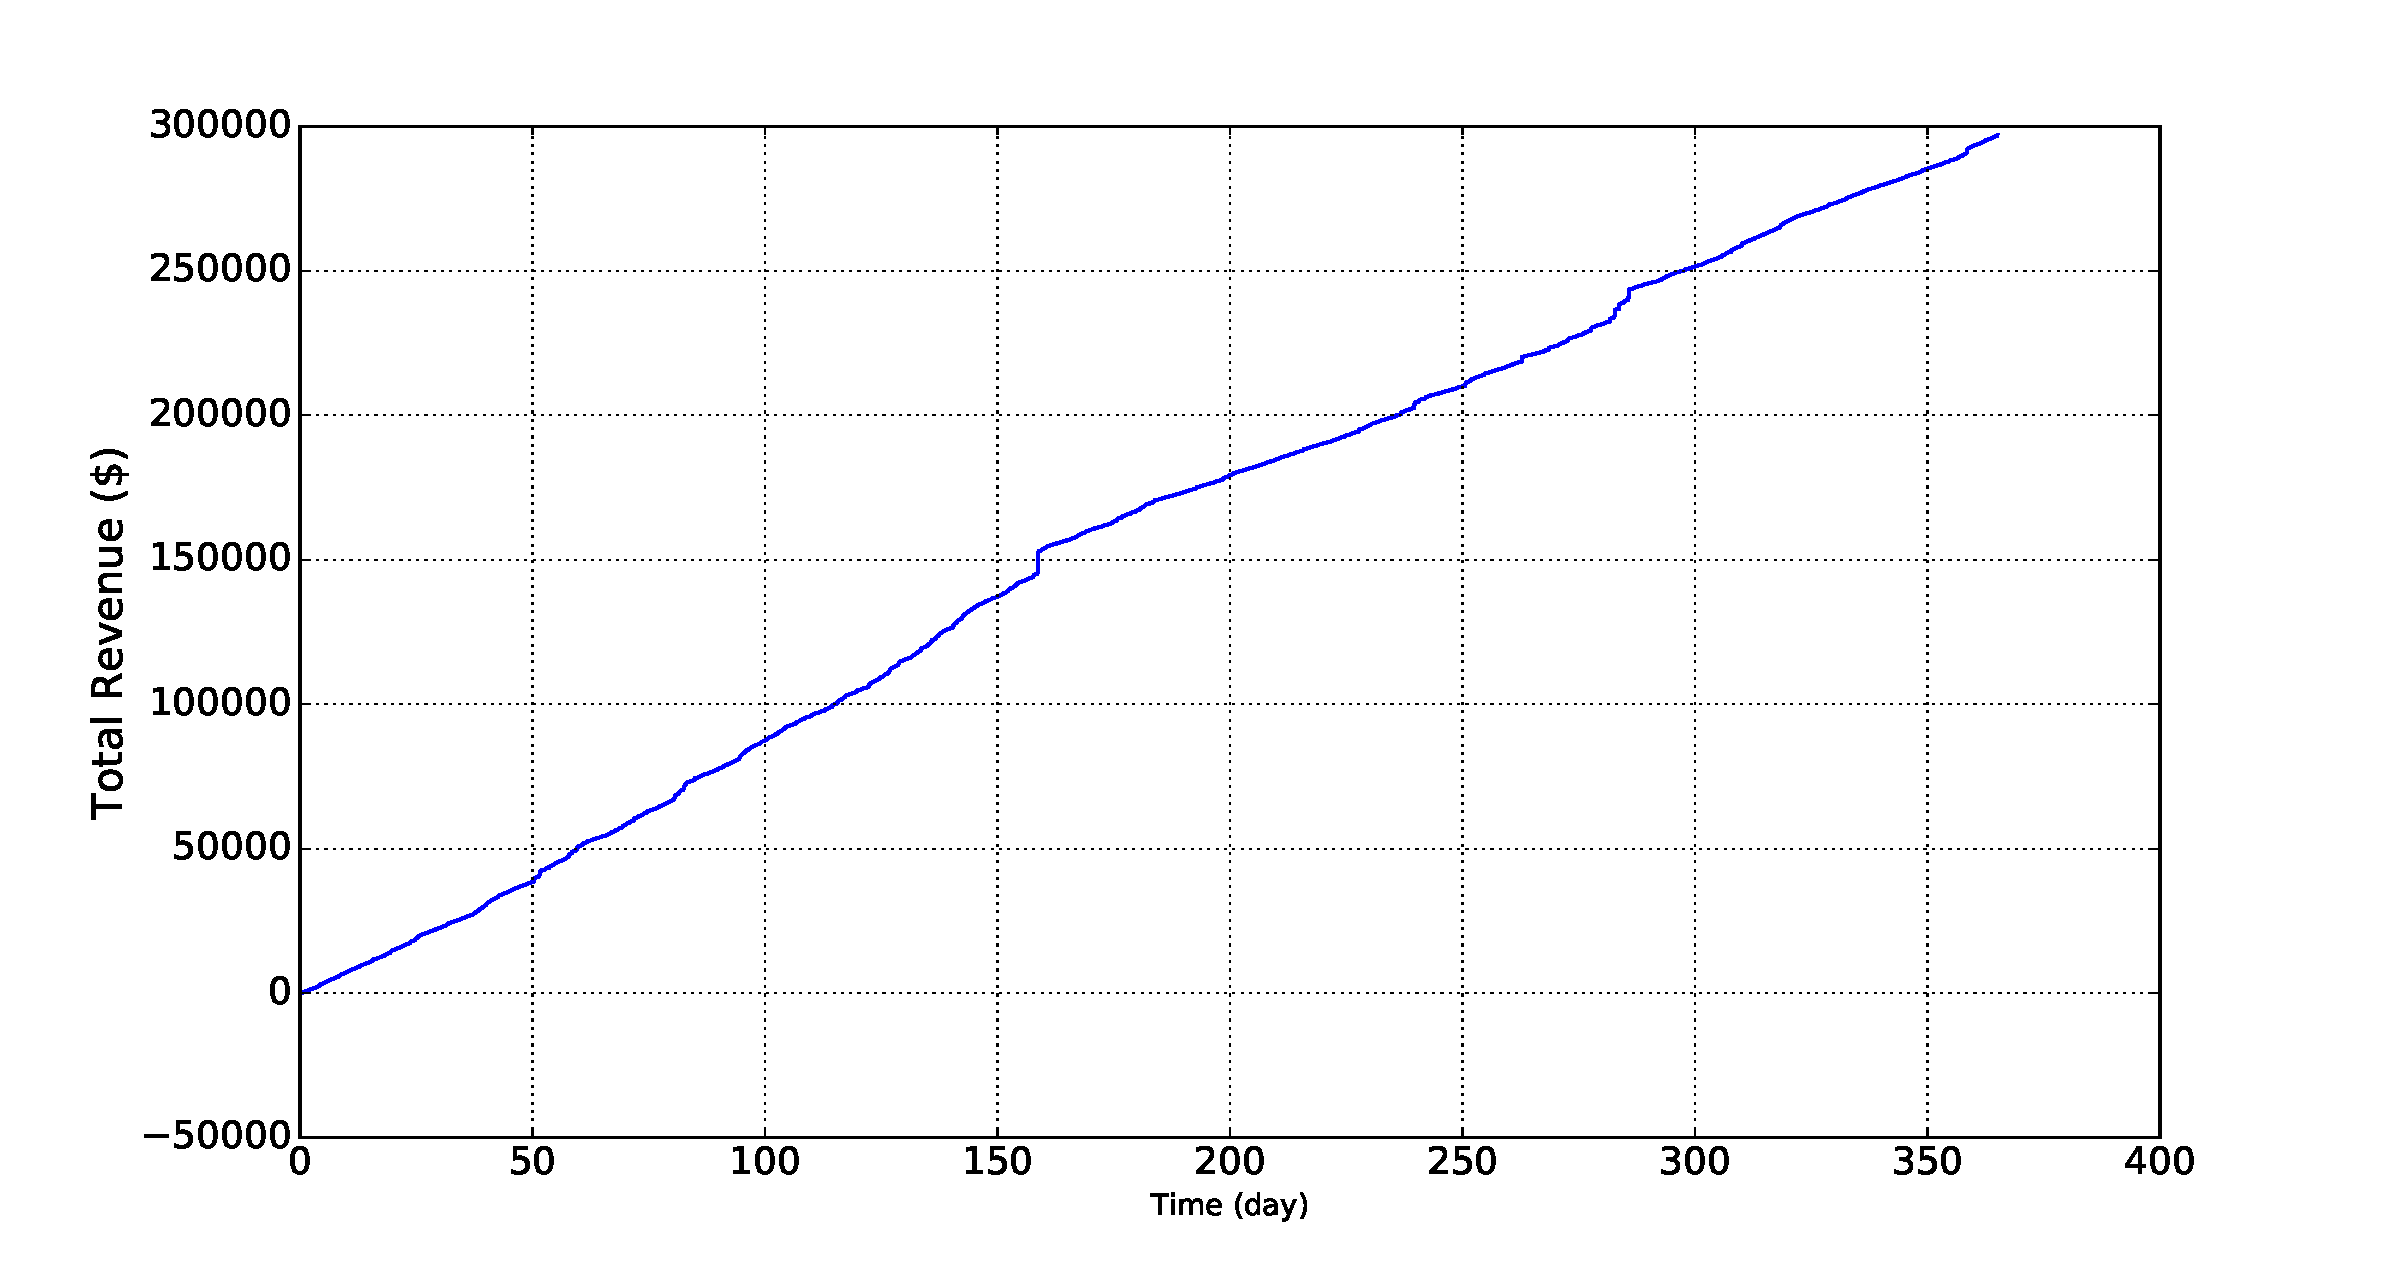
\includegraphics[width=\textwidth]{Figures/Plots/Horizon/Rev_Tot.pdf} \caption{Total revenues}\label{totrevhor}\end{subfigure} \hfill
\caption{Revenues obtained using rolling horizon approach (shown only for day 91)}\label{revhor}
\end{figure}

\section{Discussion}
\subsection{Analysis of the results}
From the Figures \ref{psim} and \ref{phor}, we observe that the battery is selling energy (and at high capacities) at all the times in the day-ahead market whereas it both buys and sells in the quarter-hourly and the real-time markets. The reason for this is that the average energy prices in the day-ahead market is higher than those in the quarter-hourly and real-time markets. So, it is more profitable for the battery to discharge by selling in the day-ahead markets and recharge by buying from the quarter-hourly and the real-time markets. Also, it is observed that it tends to buy energy at the times when the prices are lower and sell at the times when prices are higher, which also helps in maximizing the revenues. But, there are some intervals of time in which the counter-intuitive trading is done. This can be because the power is linked with the regulation up and down capacities by the constraints in Eq. \ref{eq3}. These constraints may not allow the power to follow the completely intuitive profiles because it depends on the prices of regulation up and down capacities and how much regulation capacities are being offered at those times. 

From the Figures \ref{regsim} and \ref{reghor}, we observe that the battery tends to offer maximum regulation up capacities at most of the times when the regulation up prices are high and lower regulation up capacities at the times when the regulation up prices are low. Same can be observed for regulation down capacities as well. But, this trend is not always true because of the linkage of regulation capacities with power by ythe constraints in \ref{eq3}.

Figure \ref{socsim} and \ref{sochor} just show the net effect of the power sold on the state of charge of the battery (state of charge means the fraction of battery energy out of total energy capacity of the battery). Figure \ref{pbandsim} and \ref{pbandhor} show the net bands of power within which the power grid can regulate the battery power at each interval.

Figure \ref{revsim} and \ref{revhor} show the profiles of the revenues from the energy and regulation markets throughout the year.

\subsection{Comparison of the two approaches}
We conclude that the rolling horizon approach is computationally much faster than the simultaneous approach because the single linear program for the full year becomes a huge sized problem which takes a lot of time for computations of those matrices, whereas in the rolling horizon approach each day's problem is a relatively very small problem which can be solved within milliseconds due to the small sized matrices.

Although trends of the solutions are similar, we observed that the rolling horizon approach results in slightly higher annual revenues than the simultaneous approach. By intuition this result seems to be wrong because the rolling horizon and the simultaneous approaches are two different approaches of solving the same problem. If the rolling horizon approach is giving some optimal solution, it must also be feasible in the simultaneous approach and it should also give the same solution unless there are added constraints in the simultaneous approach, which there are not any. So, this is an interesting observation and needs further investigation.

Based on our observations for the deterministic case, in which the prices for all of next 365 days were assumed to be known apriori, we expect that the rolling horizon approach will also perform much better than the simultaneous approach to solve stochastic model for this problem. In the stochastic formulation of this problem, we do not assume that the prices of the next 365 days are known. In this case, we formulate a probability distribution model for predicting the prices for next 365 days based on historical price data and then formulate the optimization model. Due to the stochasticity, the computational complexity of the problem increases and therefore, it would be very hard to solve the hugely sized problem that we get in the simultaneous approach.


\subsection{Future work}
Future work on this project can be to investigate why the revenues obtained using the rolling horizon approach are higher than that in the simultaneous approach. We need to find out whether this is a programming error or it is due to some differences in the constraints in the optimization models in the two approaches.

The next step could be to formulate the stochastic model for this problem and solve using both the approaches and compare the computational aspects of the two approaches.

Another future work would involve designing a real-time optimal controller to operate the battery in an optimal way with the rolling horizon approach, because it is computationally faster, for both deterministic and stochastic formulations.


\end{document}
